\documentclass[a4paper,12pt]{report}

% =================== PAQUETES BÁSICOS ===================
\usepackage[utf8]{inputenc}
\usepackage[T1]{fontenc}
\usepackage[spanish]{babel}
\usepackage{geometry}
\geometry{margin=2.5cm}
\usepackage{setspace}
\onehalfspacing

% =================== SUPRESIÓN DE WARNINGS DE ESPACIADO ===================
% Suprime warnings de underfull/overfull hbox (problemas de espaciado menores)
\hbadness=10000
\vbadness=10000
\hfuzz=2pt        % Tolera hasta 2pt de desbordamiento horizontal sin warning
\vfuzz=2pt        % Tolera hasta 2pt de desbordamiento vertical sin warning
\usepackage{hyperref}
\usepackage{graphicx}

% =================== SOPORTE PARA IMÁGENES SVG ===================
% Permite usar archivos SVG directamente sin necesidad de convertirlos manualmente
% NOTA: Requiere Inkscape instalado (https://inkscape.org)
% Descomenta las siguientes líneas después de instalar Inkscape:
% \usepackage{svg}
% \svgsetup{
%     inkscapearea=page,
%     inkscapelatex=false
% }
% Ruta donde se guardan las imágenes (opcional, puedes especificar una ruta específica)
\graphicspath{{recursos/}}

\usepackage{array, booktabs, longtable}
\usepackage{caption}
\usepackage{comment}
\usepackage{csquotes} % Recomendado para biblatex con babel/polyglossia
\usepackage{booktabs,subcaption,tabularx,siunitx,enumitem,pgfplots,pgfkeys,tikz}
\pgfplotsset{compat=1.18}
\usetikzlibrary{arrows.meta,positioning,shapes.geometric}
\usepackage{amssymb}
\usepackage{tikz}
\usepackage{pgfplots}
\usepackage{comment}
\usepackage{changepage}

% =================== REFERENCIAS ===================
\usepackage[backend=biber,style=ieee]{biblatex}
\addbibresource{references.bib}

% =================== ESTILO DE TÍTULOS ===================
\usepackage{titlesec}
\titleformat{\chapter}[hang]
  {\normalfont\bfseries\large\centering}   % Estilo más pequeño y centrado
  {CAPÍTULO\ \thechapter.}                 % Numeración del capítulo
  {1em}
  {\MakeUppercase}                         % Título en mayúsculas

% =================== CONFIGURACIÓN DE FLOTANTES ===================
% Mejor control de posicionamiento de figuras y tablas
\usepackage{float}
\restylefloat{table}
\restylefloat{figure}

% Parámetros para controlar la flotación
\setcounter{topnumber}{3}           % máximo 3 flotantes en la parte superior
\setcounter{bottomnumber}{2}        % máximo 2 flotantes en la parte inferior  
\setcounter{totalnumber}{4}         % máximo 4 flotantes por página
\renewcommand{\topfraction}{0.8}    % máximo 80% de la página para flotantes superiores
\renewcommand{\bottomfraction}{0.6} % máximo 60% de la página para flotantes inferiores
\renewcommand{\textfraction}{0.1}   % mínimo 10% de la página debe ser texto
\renewcommand{\floatpagefraction}{0.8} % umbral para páginas dedicadas solo a flotantes

% =================== CONFIGURACIÓN DE ÍNDICE ===================
% Mostrar hasta subsubsection (nivel 3) en la tabla de contenido

\titleformat{\section}
  {\normalfont\Large\bfseries}
  {\thesection}{1em}{}

\titleformat{\subsection}
  {\normalfont\large\bfseries}
  {\thesubsection}{1em}{}

\titleformat{\subsubsection}
  {\normalfont\normalsize\bfseries}
  {\thesubsubsection}{1em}{}
\setcounter{tocdepth}{3}
\setcounter{secnumdepth}{3}

% =================== DOCUMENTO ===================
\begin{document}
\pagenumbering{roman}
% --------- PORTADA ---------
\begin{titlepage}
    \centering

    \vspace*{1cm}

    {\LARGE\textbf{Develando al Leviatán: Proceso ágil basado en Scrum para gestionar la deuda social en el desarrollo de software ágil}}\par

    \vspace{1.5cm}

    
\includegraphics[width=0.22\textwidth]{recursos/escudoUnicauca.png}\par

    \vspace{1.0cm}

    {\large\textbf{Universidad del Cauca}} \par

    \vspace{1.5cm}

    \textbf{Luis Miguel Romero Vivas}\\
    \textbf{Manuel Santiago Córdoba Galíndez}\\


    \vspace{2.5cm}

    \textbf{Universidad del Cauca}\\
    Facultad de Ingeniería Electrónica y Telecomunicaciones\\
    \textbf{Departamento de Sistemas}\\
    Grupo de investigación en tecnologías de la información – GTI\\
    Línea de investigación ingeniería de software aplicada\\
    Popayán, marzo de 2026

\end{titlepage}


% --------- PORTADA CON DESCRIPCIÓN ------------
\begin{titlepage}
    \centering

    \vspace*{1cm}

    {\LARGE\textbf{Develando al Leviatán: Proceso ágil basado en Scrum para gestionar la deuda social en el desarrollo de software ágil}}\par

    \vspace{1.5cm}

    
\includegraphics[width=0.22\textwidth]{recursos/escudoUnicauca.png}\par

    \vspace{1.5cm}

    \textbf{Luis Miguel Romero Vivas}\\
    \textbf{Manuel Santiago Córdoba Galíndez}\\

    \vspace{1.5cm}

    Trabajo de investigación para optar al título de Ingenieros de Sistemas \par

    \vspace{1.5cm}

    \textbf{Director:} \textit{César Jesús Pardo Calvache, PhD. MS.c.} \par

    \vspace{2cm}

    \textbf{Universidad del Cauca}\\
    Facultad de Ingeniería Electrónica y Telecomunicaciones\\
    \textbf{Departamento de Sistemas}\\
    Grupo de investigación en tecnologías de la información – GTI\\
    Línea de investigación ingeniería de software aplicada\\
    Popayán, marzo de 2026

\end{titlepage}

% Página en blanco
% \clearpage
% \thispagestyle{empty}
% \null
% \clearpage

% --------- AGRADECIMIENTOS ---------
\chapter*{Agradecimientos}
\vspace{1em}
\setlength{\parindent}{0pt}

A mi familia, por su paciencia, apoyo y amor incondicional durante toda la carrera universitaria.

\vspace{1em}
A mi compañero de tesis, Manuel Santiago Córdoba Galíndez, por su colaboración, apoyo y amistad durante el desarrollo de este trabajo de grado.

\vspace{1em}
A nuestro director de tesis, el profesor PhD. MS.c. César Jesús Pardo Calvache, por su apoyo profesional y personal, su paciencia y motivación durante todo el desarrollo de este trabajo de grado.

\vspace{1em}
A mis amigos que me brindaron su apoyo, paciencia y comprensión durante este proceso.

\vspace{1em}

\begin{flushright}
    Luis Miguel Romero Vivas

    Pereira, 2026
\end{flushright}
\chapter*{Agradecimientos}
\vspace{1em}

\setlength{\parindent}{0pt}

A mi familia, por el respaldo constante, la comprensión y el cariño incondicional que me acompañaron a lo largo de toda mi formación universitaria.

\vspace{1em}
A mi compañero de tesis, Luis Miguel Romero Vivas, por su disposición, apoyo y compañerismo durante el desarrollo de este trabajo de grado.

\vspace{1em}
A nuestro director de tesis, el profesor PhD. MS.c. César Jesús Pardo Calvache, por su orientación académica, calidad humana, paciencia y motivación a lo largo de todo el proceso investigativo.

\vspace{1em}
A mis amigos, por su acompañamiento, comprensión y apoyo durante las distintas etapas de este camino.

\vspace{1em}

\begin{flushright}
    Manuel Santiago Córdoba Galíndez

    Bogotá, 2026
\end{flushright}

\clearpage
\chapter*{RESUMEN}
\addcontentsline{toc}{chapter}{\MakeUppercase{RESUMEN}}

La deuda social es un concepto que se refiere a las desigualdades y carencias que afectan a ciertos grupos dentro de una sociedad. En este contexto, el presente trabajo aborda la gestión de la deuda social mediante un enfoque ágil, proponiendo un proceso que permite identificar, priorizar y abordar las necesidades sociales de manera efectiva y eficiente.

% continúa el texto del resumen aquí
\chapter*{ABSTRACT}
\addcontentsline{toc}{chapter}{\MakeUppercase{ABSTRACT}}

This work addresses the issue of ``social debt'' in Systems Engineering, understood as the accumulation of obligations arising from interpersonal tensions, poor communication, and decisions that prioritize speed over team well-being, generating toxic environments and burnout. Despite its impact on software quality, agile frameworks such as Scrum lack systematic mechanisms to manage these human dynamics.

The objective was to define SocialScrum, an adaptation of Scrum that integrates social debt management into the technical workflow, harmonizing productivity with organizational health. The methodology was based on a Design Science Research approach. A systematic literature review was conducted to characterize ``community smells,'' and the model was designed incorporating the ``Social Guide'' role, metrics such as the ``Health Score,'' the ``Social Product Backlog,'' and ``Social Story Points.'' Conceptual validation was performed through expert judgment with six specialists in agile development, evaluating clarity, completeness, suitability, ease of use, and agility using the AgilityPRO framework.

The results indicated that SocialScrum is a clear proposal consistent with agile principles, with potential to foster collaboration without overloading the process. It is concluded that systematic social debt management is feasible, although empirical validation in real-world scenarios is required. Future work includes pilot implementation through Action Research cycles, development of tools to automate social metrics, and training programs for the proposed role.

\textbf{Keywords:} Social Debt, Agile Software Development, Scrum, SocialScrum, Design Science Research.

% --------- TABLA DE CONTENIDO Y LISTAS ---------
\renewcommand{\contentsname}{TABLA DE CONTENIDO}
\tableofcontents
\clearpage

\listoffigures
\renewcommand{\listtablename}{ÍNDICE DE TABLAS}
\renewcommand{\tablename}{Tabla}
\listoftables
\clearpage

% =================== CONTENIDO ===================
\pagenumbering{arabic}

\chapter*{CAPÍTULO 1. BASES CONCEPTUALES}
\addcontentsline{toc}{chapter}{CAPÍTULO 1. BASES CONCEPTUALES}
\setcounter{chapter}{1}
\setcounter{section}{0}
\renewcommand{\thesection}{\thechapter.\arabic{section}}
\renewcommand{\thesubsection}{\thesection.\arabic{subsection}}
\renewcommand{\thesubsubsection}{\thesubsection.\arabic{subsubsection}}

\section{Deuda social en el desarrollo de software}

La deuda social es un fenómeno que ha ganado relevancia en los equipos de desarrollo de software ágil debido a su impacto significativo y las consecuencias negativas que conlleva. Entre estas consecuencias se encuentran: la deficiente comunicación entre los miembros del equipo, el desgaste de los desarrolladores por la presión cons-tante de cumplir plazos estrictos, la falta de reconocimiento del esfuerzo individual y la ausencia de procesos de retroalimentación que dificultan la mejora continua. Según Espinosa et al. \cite{caballero2022communitysmells}, la deuda social aborda cómo las decisiones técnicas y sociales impactan los entornos de trabajo y a las personas, generándose a partir de decisiones sociotécnicas deficientes o subóptimas. En otras palabras, a medida que se toman decisiones erróneas de manera constante, los efectos negativos de la deuda social en los equipos de desarrollo de software se vuelven más pronunciados, y mientras estas malas decisiones persistan, sus efectos se intensificarán con el tiempo \cite{caballero2021thesis}.
En relación con la deuda social en el desarrollo de software ágil, existen términos asociados, como los olores comunitarios. Según Tamburri et al. \cite{tamburri2015insights}, los olores comunitarios son “conjuntos de circunstancias organizativas y sociales que tienen relaciones causales implícitas” \cite{tamburri2015insights}. Estos olores comunitarios son señales de problemas en los equipos de desarrollo de software, como conflictos entre miembros, falta de normas o procesos, o una cultura de trabajo tóxica \cite{caballero2022communitysmells}, \cite{caballero2021thesis}. Si estos problemas no se abordan, pueden conducir a la acumulación de deuda social \cite{martini2019agiledebt}.

\section{Comunicación, colaboración y coordinación (3C)}

La comunicación, colaboración y coordinación (3C) son aspectos clave al hablar de deuda social. La ausencia de estos elementos puede generar malestar en los equipos de desarrollo \cite{caballero2022communitysmells}. En cuanto a la comunicación, Saeeda et al. \cite{saeeda2024nontechnicaldebt} afirman que una comunicación efectiva es esencial para el éxito en el desarrollo de software. La adopción de atajos en la comunicación puede llevar a errores y retrasos, como omitir pasos en la recopilación de requisitos del cliente, lo que resulta en un análisis incompleto o incorrecto \cite{saeeda2024nontechnicaldebt}. De manera similar, la falta de colaboración puede tener consecuencias negativas tanto para la empresa como para los empleados. Sin una cultura de colaboración, los equipos pueden trabajar de manera aislada y descoordinada, generando errores, retrasos y menor productividad \cite{saeeda2024nontechnicaldebt}. Por último, la falta de coordinación entre los miembros del equipo puede ralentizar el progreso, aumentar los errores y reducir la productividad \cite{saeeda2024nontechnicaldebt}.

\section{Compromiso organizacional}

El compromiso organizacional es una variable clave en la gestión de la deuda social. Dignan \cite{dignan2020organizationaldebt} sostiene que la falta de compromiso por parte de la organización puede tener un impacto negativo en el desarrollo de software. Una organización ineficaz puede dificultar la comunicación y la colaboración, lo que puede llevar a errores y retrasos. Además, la falta de recursos para la implementación y mantenimiento del software puede afectar la calidad del producto final \cite{dignan2020organizationaldebt}. En situaciones como esta, es necesario un cambio. Sin embargo, como alerta Saeeda et al. \cite{saeeda2024nontechnicaldebt}, es importante prepararse para la resistencia al cambio. Para superarla, es fundamental comunicar los motivos del cambio de manera clara y convincente. Aunque los cambios importantes suelen justificarse por beneficios financieros, es crucial que las personas comprendan cómo estos beneficios se traducen en ventajas tangibles para ellos \cite{saeeda2024nontechnicaldebt}.

\section{Síndrome de Burnout}

El síndrome de Burnout es un problema frecuente en el desarrollo de software ágil y afecta gravemente a las personas. Según Tulili et al. \cite{tulili2022burnout}, el síndrome de Burnout es el agotamiento mental, físico y emocional provocado por factores relacionados con el trabajo. Los factores más comunes incluyen la tensión y el control en el trabajo, la sobrecarga laboral, el conflicto de roles, la especialización del trabajo y las exigencias laborales \cite{tulili2022burnout}. Otros estudios han identificado factores adicionales que contribuyen al Burnout, como la sobrecarga de información, la cascada de datos, largas rachas de contribuciones ininterrumpidas y las tensiones laborales prolongadas derivadas de la pandemia de COVID-19 \cite{tulili2022burnout}. Al ser un problema que afecta directamente a las personas, el síndrome de Burnout puede generar deuda social y, por lo tanto, debe considerarse al gestionar esta deuda.

\section{Goal Question Metric (GQM)}

Es una metodología estructurada para definir y evaluar métricas de software alineadas con los objetivos organizacionales. Desarrollado por Victor R. Basili, Gianluigi Caldiera y H. Dieter Rombach en 1994 \cite{caldiera1994gqm}, este enfoque se basa en tres niveles: definir metas claras y específicas (Goal), formular preguntas que ayuden a evaluar si se están alcanzando las metas (Question) e identificar y recolectar datos que respondan a estas preguntas (Metric). El GQM permite a las organizaciones medir de manera efectiva e interpretar los datos en función de sus objetivos, mejorando así la calidad del software a través de prácticas de medición sistemáticas.

\section{Scrum}

Scrum es un marco de trabajo que ayuda a las personas, equipos y organizaciones a generar valor a través de soluciones adaptativas para problemas complejos; donde su arquitectura en equipos reducidos y autogestionados operan mediante ciclos iterativos —denominados Sprints—, los cuales, tiene una duración máxima de un mes, priorizando la entrega iterativa de valor. En Scrum, tres roles vertebran su estructura: el Scrum Master, que facilita los procesos; el Product Owner, el responsable del valor; y el Equipo de Desarrollo, ejecutores de tareas. Su núcleo operativo reside en la tríada de transparencia-inspección-adaptación. En eventos estructurados tenemos el Sprint Planning, Daily Scrum, Sprint Review y Sprint Retrospective \cite{schwaber2020scrum}. Cabe subrayar que, a diferencia de otras metodologías, Scrum no prescribe herramientas técnicas específicas; su esencia radica en proveer un esqueleto mínimo que catalice la colaboración y la mejora progresiva \cite{takeuchi1986new}.
\chapter*{CAPÍTULO 2. Marco teórico y trabajos relacionados}
\addcontentsline{toc}{chapter}{CAPÍTULO 2. Marco teórico y trabajos relacionados}
\setcounter{chapter}{2}
\setcounter{section}{0}
\setcounter{subsection}{0}
\setcounter{subsubsection}{0}
\setcounter{figure}{0}
\setcounter{table}{0}
\renewcommand{\thesection}{\thechapter.\arabic{section}}
\renewcommand{\thesubsection}{\thesection.\arabic{subsection}}
\renewcommand{\thesubsubsection}{\thesubsection.\arabic{subsubsection}}
\makeatletter
\protected@edef\@currentlabel{\thechapter}%
\makeatother
\label{chap:capitulo2}

En este capítulo se presentan las bases conceptuales que sustentan la investigación y los trabajos relacionados identificados mediante una \acrfull{rsl}. En la primera sección se abordan los conceptos clave relacionados con la deuda social, el síndrome de Burnout, el marco de trabajo \gls{scrum} y la \gls{dsr}. En la segunda sección se describe el protocolo de investigación de la RSL, los hallazgos más relevantes y las brechas existentes que motivan la propuesta de \gls{socialscrum}.

% ------- SECCIÓN 1: DEUDA SOCIAL EN EL DESARROLLO DE SOFTWARE -------
\section{Marco teórico}
\subsection{Deuda social en el desarrollo de software}

La \gls{deuda-social} se describe como la acumulación de costos imprevistos, o potenciales costos, en proyectos de software, generando así un conjunto de decisiones sociotécnicas deficientes que resultan de procesos de desarrollo subóptimos \cite{caballero2022communitysmells}. Dicho de otro modo, a medida que se toman decisiones erróneas de manera constante, los efectos negativos de la deuda social en los equipos de desarrollo de software se vuelven más pronunciados, y mientras estas malas decisiones persistan, sus efectos se intensificarán con el tiempo \cite{caballero2021thesis}. Este concepto, que proviene de la sociología —donde originalmente se usaba para explicar cómo las obligaciones sociales pueden afectar las relaciones interpersonales— ha sido adoptado por los investigadores en ingeniería de software para describir fenómenos similares dentro de los equipos de desarrollo y sus organizaciones \cite{caballero2022communitysmells}.

\subsubsection{Analogía y distinción con la deuda técnica}
La deuda social es, en muchos sentidos, análoga a la deuda técnica \cite{tamburri2015insights}. Ambas representan el estado de las organizaciones de software como resultado de decisiones acumuladas —que, si bien pueden ofrecer beneficios a corto plazo— generan un ``interés'' que se manifiesta como costos adicionales a medio y largo plazo \cite{martini2019agiledebt}. No obstante, existe una diferencia fundamental:
\begin{itemize}
    \item La deuda técnica se centra en decisiones técnicas postergadas, como refactorizaciones de código o decisiones arquitectónicas que afectan la calidad del software \cite{caballero2022communitysmells}.
    \item En contraste, la deuda social se enfoca en decisiones sociotécnicas incorrectas que moldean el entorno de trabajo y que influyen directamente en el bienestar, las interacciones sociales y el rendimiento de los desarrolladores \cite{caballero2022communitysmells}, \cite{caballero2021thesis}. Por lo tanto, mientras la deuda técnica se ocupa de la parte técnica del software, la deuda social pone el foco en las ``personas''. Cabe señalar que, de forma recíproca, la deuda social puede ser una causa subyacente de la deuda técnica \cite{caballero2022communitysmells}, \cite{caballero2021thesis}.
\end{itemize}

\subsubsection{Community smells (olores comunitarios)}
La acumulación de deuda social se inicia con una o más decisiones sociotécnicas equivocadas \cite{caballero2022communitysmells}. La presencia de \gls{community-smells} es un indicador clave de que algo no funciona correctamente dentro de los equipos \cite{caballero2022communitysmells}. Estos olores comunitarios son, en esencia, antipatrones sociotécnicos \cite{caballero2022communitysmells}, definidos como ``conjuntos de circunstancias organizacionales y sociales, con relaciones causales implícitas’’ \cite{caballero2022communitysmells}, \cite{tamburri2015insights}. Cuando estos olores comunitarios persisten, se genera una acumulación de deuda social \cite{caballero2022communitysmells}. Las fuentes identificadas de estos olores comunitarios son diversas y se manifiestan a través de modelos de causa y efecto, por ejemplo:
\begin{itemize}
    \item Decisiones inadecuadas de gestión de la información que resultan en una arquitectura por ósmosis, donde los desarrolladores no tienen acceso a información arquitectónica clave, lo que lleva a la frustración y al desperdicio de tiempo \cite{caballero2022communitysmells}.
    \item Problemas de coordinación de tareas en equipos aislados, conocidos como \gls{cs-org-silo}, que dificultan la comunicación y la cooperación efectiva \cite{caballero2022communitysmells}.
    \item Comportamientos individuales desafiantes, como el \gls{cs-lone-wolf} donde un desarrollador trabaja de forma independiente sin comunicarse con sus compañeros, generando decisiones arquitectónicas no sancionadas y retrasos en el proyecto \cite{caballero2022communitysmells}.
    \item Estructuras organizacionales excesivamente formales o complejas que dan lugar al \gls{cs-radio-silence} o \gls{cs-bottleneck}, creando cuellos de botella en la comunicación y retrasos masivos. Dichos olores comunitarios impactan principalmente en las emociones, estresan las interacciones sociales, afectan el rendimiento del equipo y disminuyen la calidad del software \cite{caballero2022communitysmells}.
\end{itemize}

\subsubsection{El impacto de la deuda social en el entorno ágil}
La deuda social tiene un impacto profundo y multifacético en los equipos de desarrollo ágil y sus organizaciones \cite{caballero2022communitysmells}. Entre las consecuencias más notables se incluyen:
\begin{itemize}
    \item Reacciones humanas adversas y un deterioro del bienestar de los individuos \cite{caballero2022communitysmells}.
    \item Relaciones sociales tensas y conflictos entre compañeros de trabajo, lo que afecta la cohesión del equipo \cite{caballero2022communitysmells}.
    \item Bajo rendimiento del equipo y prácticas de trabajo subóptimas que afectan la calidad del software \cite{caballero2022communitysmells}.
    \item Artefactos de software defectuosos y productos de baja calidad que no cumplen con las expectativas del cliente \cite{caballero2022communitysmells}.
    \item El impacto económico no se limita a simples cifras: suele traducirse en gastos inesperados que, en algunos casos, pueden amenazar la continuidad misma del negocio \cite{caballero2022communitysmells}. Esto cobra especial relevancia en entornos de proyectos ágiles a gran escala (LSA), donde diversos equipos autónomos colaboran en pos de un objetivo común. En estos escenarios, la coordinación y una gestión eficaz no son opcionales, sino piezas clave para mantener el rumbo \cite{martini2019agiledebt}. Una alta autonomía de equipo, si no se equilibra con una alineación adecuada, puede llevar a procesos subóptimos que generen deuda social, como duplicación de trabajo o problemas de integración \cite{martini2019agiledebt}. Como documentan Martini \textit{et al.} \cite{martini2019agiledebt}, la deuda social se manifiesta en discusiones sobre autonomía del equipo, la implicación del liderazgo y la comunicación entre equipos.
\end{itemize}

\subsubsection{Desafíos en la medición y gestión de la deuda social}
Pese a su clara importancia, los investigadores aún enfrentan el desafío de expresar los efectos de la deuda social en términos monetarios precisos \cite{caballero2022communitysmells}. Aunque marcos como DAHLIA \cite{caballero2022communitysmells}, \cite{tamburri2019software} han intentado cuantificar la deuda social, principalmente en relación con la ininteligibilidad arquitectónica, se requiere más investigación empírica para generalizar estas medidas a la vasta gama de olores comunitarios \cite{caballero2022communitysmells}. Por lo tanto, las organizaciones necesitan abordar las decisiones sociotécnicas deficientes y ``saldar'' esta deuda social a través de estrategias de gestión que incluyen enfoques organizacionales, marcos, modelos, herramientas y directrices \cite{caballero2022communitysmells}.

% ------- SECCIÓN 2: SÍNDROME DE BURNOUT -------

\subsection{Síndrome de Burnout}

El Síndrome de \Gls{burnout}, descrito inicialmente en 1974 por el psicólogo Herbert Freudenberger \cite{tulili2022burnout}, es un síndrome relacionado con el trabajo que se manifiesta como agotamiento emocional, despersonalización, sobrecarga laboral y una percepción de escasez de logros personales \cite{tulili2022burnout}. Como bien señalan las investigaciones, su alcance trasciende ámbitos específicos —arquitectura, sector educativo, administración pública o ventas— \cite{tulili2022burnout} para manifestarse como un fenómeno epidémico en entornos STEM (Science, Technology, Engineering y Mathematics). Dicho de otro modo, su omnipresencia y sus repercusiones son un factor crítico que obstaculiza el avance profesional y subyace al estrés laboral en los diversos campos en general \cite{tulili2022burnout}.
En la ingeniería de software (SE) y, sobre todo con respecto a la deuda social, el burnout no es una excepción. De hecho, informes recientes, especialmente tras la pandemia de COVID-19, han puesto de manifiesto que más del 80~\% de los desarrolladores encuestados han experimentado o están experimentando alguna forma de burnout \cite{tulili2022burnout}. La Organización Mundial de la Salud (OMS) ha clasificado el burnout como un fenómeno ocupacional en las ediciones 10ª y 11ª de la Clasificación Internacional de Enfermedades (ICD-10, ICD-11), lo que intensifica su gravedad y el reconocimiento de su impacto en la salud mental en el ámbito laboral \cite{tulili2022burnout}.
Los estudios han explorado a fondo las causas y consecuencias del burnout entre los equipos de desarrollo. Las consecuencias fundamentales reportadas del burnout incluyen:
\begin{itemize}
    \item \textbf{Agotamiento:} La sensación de estar abrumado y exhausto de recursos emocionales y físicos \cite{tulili2022burnout}.
    \item \textbf{Cinismo:} Una actitud negativa, hostil y excesivamente distante hacia el trabajo y los compañeros \cite{tulili2022burnout}.
    \item \textbf{Ineficacia profesional:} La percepción de una disminución en la competencia, el logro personal y productividad en el trabajo \cite{tulili2022burnout}.
\end{itemize}
No obstante, al considerar el burnout como un síntoma de ``deuda social’’, nuestra atención se dirige hacia las dinámicas subyacentes y las expectativas tácitas o explícitas no satisfechas dentro de las interacciones humanas y organizacionales. El burnout en la deuda social sí describe fenómenos que encajan con esta interpretación; por ejemplo, las prácticas de comunicación deficientes son una causa recurrente de burnout:
\begin{itemize}
    \item Una menor participación de los empleados en la comunicación organizacional se correlaciona con un mayor agotamiento emocional \cite{tulili2022burnout}.
    \item La apertura a la crítica puede causar burnout si no se maneja adecuadamente, ya que la falta de retroalimentación constructiva puede llevar a la frustración y al agotamiento emocional \cite{tulili2022burnout}.
    \item Los problemas de comunicación entre gerentes y miembros del equipo, así como los desacuerdos entre compañeros, han sido señalados como factores desencadenantes del burnout \cite{tulili2022burnout}.
\end{itemize}
Teniendo en cuenta lo descrito anteriormente, las relaciones tóxicas en equipos de desarrollo son claros detonantes de burnout. Como demuestran estudios recientes, el lenguaje descortés en comunicaciones técnicas (desde ``solicitudes agresivas’’ hasta comentarios despectivos) erosiona la confianza y genera una deuda social acumulada: ese déficit invisible de respeto y apoyo mutuo que pagamos con estrés crónico \cite{tulili2022burnout}.
Paralelamente, factores como sobrecarga laboral, roles ambiguos o tecnoestrés —estrés causado por la tecnología— aíslan a los profesionales, impidiéndoles conectar con sus equipos \cite{tulili2022burnout}. Cuando la presión ahoga la interacción humana, germina el cinismo y la despersonalización —síntomas clave del burnout. Esta desconexión representa otra deuda organizacional: la que se contrae al sacrificar el bienestar por la productividad inmediata \cite{tulili2022burnout}.
El desenlace es amargo: ese profesional agotado que abandona la carrera no solo reduce la productividad, sino que cobra simbólicamente la deuda social acumulada. Su partida es el recordatorio más crudo de que ningún proyecto sobrevive cuando quema a su gente \cite{tulili2022burnout}.

% ------- SECCIÓN 3: SCRUM -------

\subsection{Scrum}
\subsubsection{Definición de Scrum}
Scrum es un marco de trabajo ligero que ayuda a las personas, equipos y organizaciones a generar valor a través de soluciones adaptativas para problemas complejos \cite{schwaber2020scrum}. Concebido originalmente por Takeuchi y Nonaka \cite{takeuchi1986new} como una analogía del rugby para describir equipos multifuncionales que avanzan juntos, Scrum fue formalizado como proceso de desarrollo de software por Schwaber y Sutherland a mediados de la década de 1990 y ha sido actualizado progresivamente hasta la Scrum Guide 2020 \cite{schwaber2020scrum}.

Su arquitectura se basa en equipos reducidos y autogestionados que operan mediante ciclos iterativos denominados \textit{Sprints}, con una duración máxima de un mes, priorizando la entrega incremental de valor. A diferencia de otras metodologías, Scrum no prescribe herramientas técnicas específicas; su esencia radica en proveer un esqueleto mínimo que catalice la colaboración y la mejora progresiva \cite{takeuchi1986new}.

\subsection{Ciencia del Diseño (Design Science Research)}
\label{sec:dsr}

La investigación de la \gls{dsr} es un paradigma de investigación ampliamente reconocido en los sistemas de información y la ingeniería de software, cuyo objetivo central es la creación y evaluación rigurosa de artefactos como modelos, métodos, constructos o instancias, que resuelvan problemas organizacionales identificados \cite{hevner2004designscience}. A diferencia de las ciencias del comportamiento, que buscan describir y explicar fenómenos, la DSR se orienta a \textit{prescribir} soluciones innovadoras, evaluando su utilidad y eficacia mediante procesos iterativos de diseño y validación.

Peffers \textit{et al.} \cite{peffers2007dsrm} proponen un modelo de proceso ampliamente adoptado que estructura la DSR en seis fases: (1) identificación del problema y motivación, (2) definición de los objetivos de la solución, (3) diseño y desarrollo del artefacto, (4) demostración, (5) evaluación, y (6) comunicación de resultados. Una característica clave de este modelo es que la evaluación del artefacto puede realizarse de múltiples formas desde la evaluación conceptual por expertos hasta la experimentación empírica en contextos reales dependiendo del grado de madurez del artefacto y de las restricciones del entorno de investigación.

Wieringa \cite{wieringa2014dsr} amplía esta perspectiva al distinguir entre la validación previa a la implementación y la validación posterior a la implementación en un contexto real. Esta distinción resulta especialmente relevante para la presente investigación, ya que SocialScrum involucra variables sensibles de salud mental y clima laboral, lo que justifica la realización de una validación conceptual rigurosa como paso previo y necesario antes de una intervención empírica en equipos de desarrollo reales.

En el contexto de esta tesis, la DSR proporciona el marco metodológico que guía la construcción y evaluación del artefacto SocialScrum. Las fases ejecutadas (identificación del problema mediante RSL, diseño y construcción del modelo, evaluación mediante juicio de expertos y comunicación de resultados) se corresponden con las etapas del proceso de Peffers \textit{et al.} \cite{peffers2007dsrm}, como se detalla en la Sección~\ref{sec:metodo-investigacion} del Capítulo~\ref{chap:capitulo1}.

\section{Trabajos relacionados}
A continuación, se presentan algunos hallazgos documentados en la \acrfull{rsl} realizada, que identifican las brechas existentes, los objetivos del proyecto y los aportes encontrados. La RSL se llevó a cabo siguiendo el protocolo detallado en \cite{jalali2012systematic} y \cite{palomba2021communitysmells}, que incluye las siguientes actividades: (i) aplicación del enfoque GQM (Goal-Question-Metric) \cite{caldiera1994gqm} y el marco de trabajo S.M.A.R.T (Specific, Measurable, Achievable, Realistic, Time-bound) \cite{Doran1981}, (ii) definición de la estrategia de búsqueda y selección, (iii) realización de la revisión, y (iv) elaboración del informe de la revisión. La RSL completa está disponible en el Anexo A. Este proceso se realizó con el objetivo de recopilar y categorizar la información existente sobre el tema de investigación. A continuación, en la Figura \ref{fig:smart-gqm} se puede observar la secuencia de actividades realizadas para la RSL:

\begin{figure}[!htbp]
    \centering
    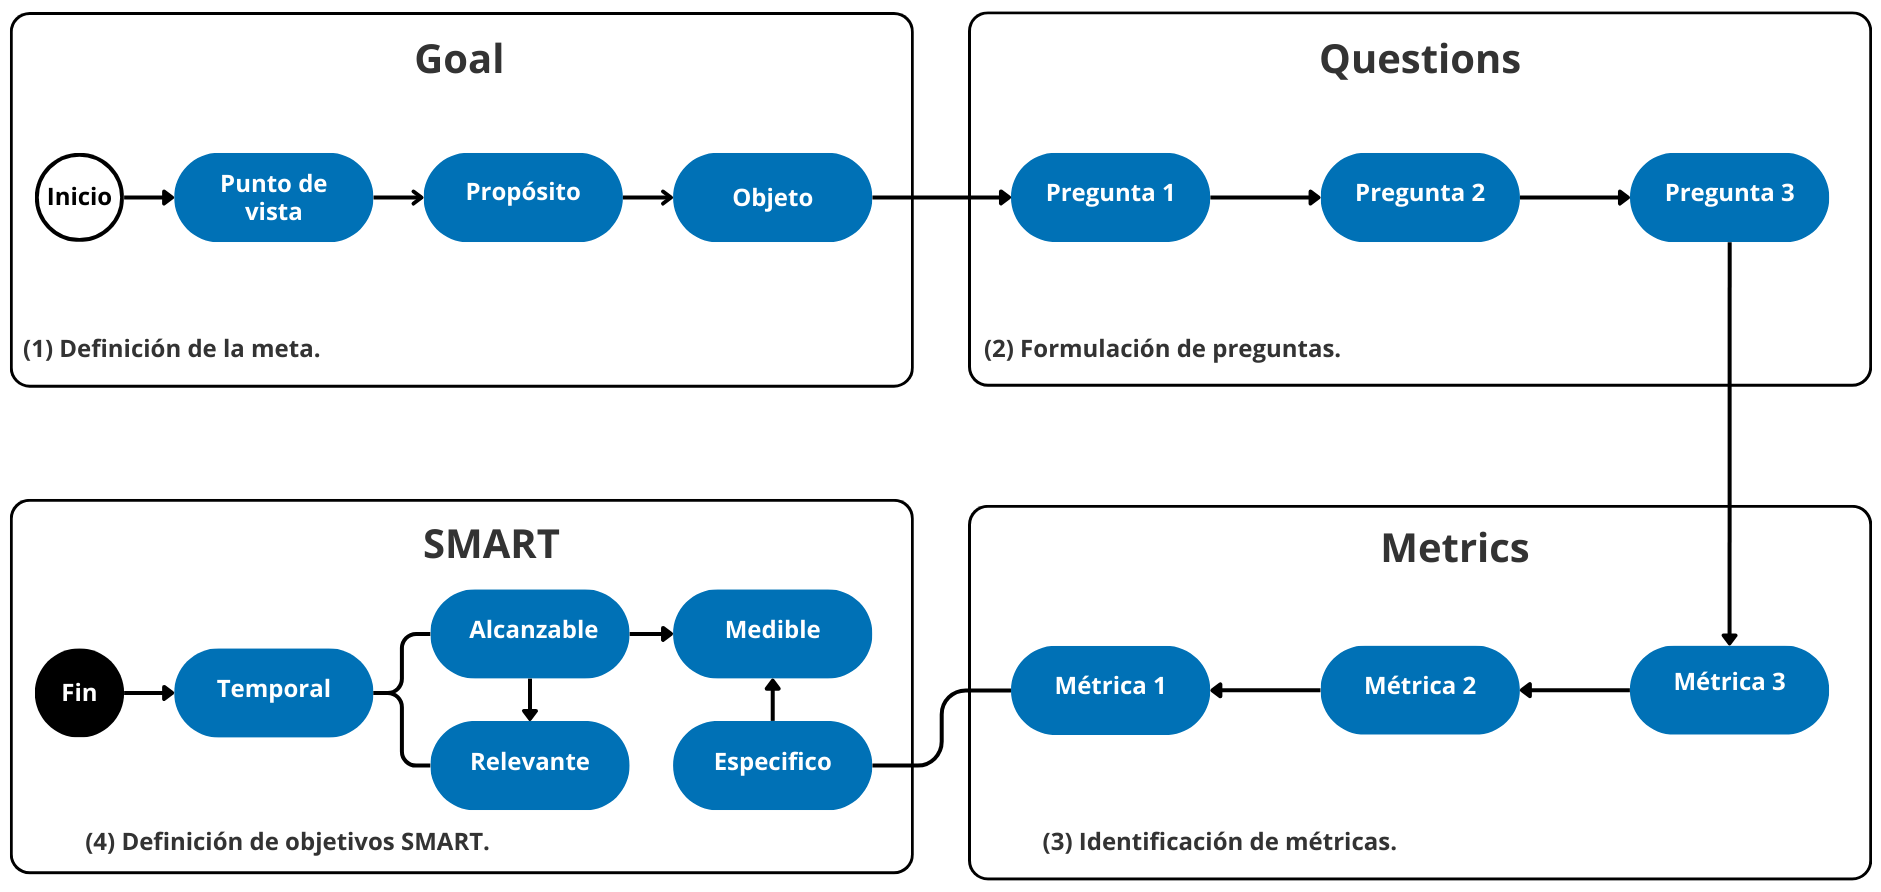
\includegraphics[width=1.0\textwidth]{recursos/capitulo2/smart-gqm.png}
    \caption{Secuencia de actividades realizadas para la RSL}
    \label{fig:smart-gqm}
\end{figure}

\subsection{Protocolo de investigación}
Para llevar a cabo la RSL, se utilizaron herramientas tecnológicas de inteligencia artificial, como ChatGPT \cite{openai2022chatgpt} y Microsoft Copilot \cite{microsoft2023copilot}, con el objetivo de obtener diversas formas de definir un mismo concepto y construir la cadena de búsqueda básica. Los documentos a menudo presentan temas de manera dispersa y poco clara, lo que puede generar sesgos y dudas. En este contexto, las herramientas de IA generativa resultaron ser recursos valiosos, ya que, mediante prompts específicos, permitieron iniciar conversaciones y obtener información más precisa. A partir de los términos identificados con la ayuda de estas herramientas, se definió una versión inicial de la cadena de búsqueda básica: ``social debt'' OR ``social software engineering'' AND ``agile software development'' OR ``software development teams''.
Posteriormente, se seleccionó Google Scholar como la base de datos principal para obtener información o estudios relacionados. Esta elección se basó en varias razones:
\begin{itemize}
    \item Amplia cobertura: Google Scholar indexa una gran variedad de fuentes académicas, incluyendo artículos, tesis, libros y conferencias, lo que permite acceder a una amplia gama de literatura relevante.
    \item Accesibilidad: Es una herramienta de acceso abierto y gratuito, lo que facilita su uso para investigadores con recursos limitados.
    \item Relevancia: Google Scholar utiliza algoritmos que priorizan artículos altamente citados y relevantes, lo que ayuda a identificar estudios influyentes en el campo de la deuda social y el desarrollo ágil.
    \item Integración con otras bases de datos: Aunque Google Scholar fue la base principal, también se complementó con otras bases de datos especializadas, como IEEE Xplore, SpringerLink y Science Direct, para asegurar una revisión exhaustiva.
\end{itemize}
La búsqueda manual reveló que las frases clave ``social debt'' y ``agile software development'' eran esenciales para definir la cadena de búsqueda básica. Por esta razón, se decidió utilizar el conector lógico ``AND'' para unir estas dos frases, ya que los artículos relevantes para la investigación las mencionaban conjuntamente. De esta manera, la cadena de búsqueda básica: ``social debt'' AND ``agile software development'' se aplicó inicialmente a seis bases de datos científicas: Google Scholar, IEEE Xplore, SpringerLink y Science Direct, como se observa en la Tabla \ref{tab:cadenas-busqueda}.

\begingroup
\scriptsize % Fuente ligeramente reducida
\setlength{\LTleft}{0pt} % Alinear tabla a la izquierda
\setlength{\LTright}{0pt} % Permitir que la tabla ocupe espacio a la derecha
\setlength{\tabcolsep}{4pt} % Ajuste de espacio entre columnas
\renewcommand{\arraystretch}{1.4} % Mayor espacio entre filas para facilitar la lectura

\begin{longtable}[H]{|
    >{\Centering\hspace{0pt}}p{0.8cm}|      % Col 1: No.
    >{\RaggedRight\hspace{0pt}}p{9.6cm}|    % Col 2: Cadena de búsqueda 
    >{\Centering\hspace{0pt}}p{2.5cm}|      % Col 3: Fuente 
    >{\Centering\hspace{0pt}}p{2.0cm}|      % Col 4: Estado 
    }

    % --- 1. ENCABEZADO PARA LA PRIMERA PÁGINA ---
    \caption{Cadenas de búsqueda utilizadas en la revisión sistemática} \label{tab:cadenas-busqueda}                                        \\
    \hline
    \textbf{No.} & \textbf{Cadena de búsqueda}                                                          & \textbf{Fuente} & \textbf{Estado} \\
    \hline
    \endfirsthead

    % --- 2. ENCABEZADO PARA PÁGINAS SIGUIENTES ---
    \hline
    \multicolumn{4}{|c|}{{\bfseries \tablename\ \thetable{} -- Continuación}}                                                               \\
    \hline
    \textbf{No.} & \textbf{Cadena de búsqueda}                                                          & \textbf{Fuente} & \textbf{Estado} \\
    \hline
    \endhead

    % --- 3. PIE PARA PÁGINAS INTERMEDIAS ---
    \hline
    \multicolumn{4}{|r|}{\textit{Continúa en la siguiente página...}}                                                                       \\
    \hline
    \endfoot

    % --- 4. PIE FINAL ---
    \hline
    \multicolumn{4}{|l|}{\footnotesize \textit{Acrónimos utilizados: Identificador (No)}}                                                   \\
    \hline
    \endlastfoot

    % --- CONTENIDO ---
    1            & ``social debt'' AND ``agile software development''                                   & Google Scholar  & Incluida        \\
    \hline
    2            & (``Full Text Only'':social debt) AND (``Full Text Only'':agile software development) & IEEE Xplore     & Incluida        \\
    \hline
    3            & ‘‘social debt’ AND ‘agile software development’’                                     & SpringerLink    & Incluida        \\
    \hline
    4            & ‘social debt’ AND ‘agile software development’                                       & Science Direct  & Incluida        \\
\end{longtable}
\endgroup



La cadena de búsqueda se aplicó a una ventana de tiempo desde 2013 hasta 2024, adaptándose a los filtros y parámetros específicos de cada motor de búsqueda. Tras realizar las modificaciones necesarias a la cadena de búsqueda básica, se inició la búsqueda en cada motor. La Tabla \ref{tab:resultados-busqueda-longtable} muestra el total de artículos encontrados, relevantes, repetidos y primarios.

\begingroup
\scriptsize % Fuente ligeramente reducida
\setlength{\LTleft}{0pt} % Alinear tabla a la izquierda
\setlength{\LTright}{0pt} % Permitir que la tabla ocupe espacio a la derecha
\setlength{\tabcolsep}{5pt} % Ajuste de espacio entre columnas
\renewcommand{\arraystretch}{1.4} % Mayor espacio entre filas
\begin{longtable}[H]{|
    >{\Centering\hspace{0pt}}p{0.8cm}|   % Col 1: No.
    >{\RaggedRight\hspace{0pt}}p{4.8cm}| % Col 2: Motor de búsqueda (Aumentado para llenar ancho)
    >{\Centering\hspace{0pt}}p{1.8cm}|   % Col 3: Encontrados
    >{\Centering\hspace{0pt}}p{1.8cm}|   % Col 4: Relevantes
    >{\Centering\hspace{0pt}}p{2.2cm}|   % Col 5: Relevantes repetidos
    >{\Centering\hspace{0pt}}p{2.5cm}|   % Col 6: Primarios seleccionados
    }
    % --- CÁLCULO DE ANCHOS ---
    % Objetivo: ~16.5 - 17cm (Ancho texto A4 típico con márgenes 2.5cm)
    % -------------------------

    % Encabezado primera página
    \caption{Resultados por motor de búsqueda en la revisión sistemática} \label{tab:resultados-busqueda-longtable}                                           \\
    \hline
    \textbf{No.} & \textbf{Motor de búsqueda} & \textbf{Encontrados} & \textbf{Relevantes} & \textbf{Relevantes repetidos} & \textbf{Primarios seleccionados} \\
    \hline
    \endfirsthead

    % Encabezado páginas siguientes
    \hline
    \multicolumn{6}{|c|}{{\bfseries \tablename\ \thetable{} -- Continuación}}                                                                                 \\
    \hline
    \textbf{No.} & \textbf{Motor de búsqueda} & \textbf{Encontrados} & \textbf{Relevantes} & \textbf{Relevantes repetidos} & \textbf{Primarios seleccionados} \\
    \hline
    \endhead

    % Pie páginas intermedias
    \hline
    \multicolumn{6}{|r|}{\textit{Continúa en la siguiente página...}}                                                                                         \\
    \hline
    \endfoot

    % Pie final
    \hline
    \multicolumn{6}{|l|}{\footnotesize \textit{Acrónimos utilizados: Identificador (No)}}                                                                     \\
    \hline
    \endlastfoot

    % CONTENIDO
    1            & Google Scholar             & 130                  & 15                  & 0                             & 8                                \\
    \hline
    2            & IEEE Xplore                & 28                   & 3                   & 0                             & 0                                \\
    \hline
    3            & Science Direct             & 5                    & 0                   & 0                             & 0                                \\
    \hline
    4            & SpringerLink               & 35                   & 2                   & 0                             & 0                                \\
    \hline
                 & \textbf{Total}             & \textbf{198}         & \textbf{20}         & \textbf{0}                    & \textbf{8}                       \\
\end{longtable}
\endgroup


En la Tabla \ref{tab:preguntas-investigacion-longtable} se presentan las preguntas de investigación definidas que ayudaron a segmentar la información identificada en los artículos primarios, su motivación y la relación que tienen con los objetivos propuestos en la RSL. Debido a la limitación de espacio, la RSL se puede consultar en detalle en el Anexo~\ref{anexo:a}.

\begingroup
\scriptsize
\setlength{\LTleft}{0pt} % Alinear tabla a la izquierda
\setlength{\LTright}{0pt} % Permitir que la tabla ocupe espacio a la derecha
\setlength{\tabcolsep}{4pt} % Ajuste de espacio entre columnas
\renewcommand{\arraystretch}{1.4}

\begin{longtable}[H]{|
    >{\Centering\hspace{0pt}}p{0.7cm}|     % Id.
    >{\RaggedRight\hspace{0pt}}p{8.0cm}|   % Pregunta de investigación
    >{\RaggedRight\hspace{0pt}}p{6.5cm}|   % Motivación
    }

    % --- ENCABEZADO PRIMERA PÁGINA ---
    \caption{Preguntas de investigación definidas}
    \label{tab:preguntas-investigacion-longtable}                                                                                                                                                                                                                           \\
    \hline
    \textbf{Id.}                                                                                                                                                                                                 & \textbf{Pregunta de investigación} & \textbf{Motivación} \\
    \hline
    \endfirsthead

    % --- ENCABEZADO PÁGINAS SIGUIENTES ---
    \hline
    \multicolumn{3}{|c|}{{\bfseries \tablename\ \thetable{} -- Continuación}}                                                                                                                                                                                               \\
    \hline
    \textbf{Id.}                                                                                                                                                                                                 & \textbf{Pregunta de investigación} & \textbf{Motivación} \\
    \hline
    \endhead

    % --- PIE PÁGINAS INTERMEDIAS ---
    \hline
    \multicolumn{3}{|r|}{\textit{Continúa en la siguiente página...}}                                                                                                                                                                                                       \\
    \hline
    \endfoot

    % --- PIE FINAL ---
    \hline
    \multicolumn{3}{|l|}{\footnotesize \textit{Acrónimos utilizados: Identificador (Id), Pregunta de investigación (PI)}}                                                                                                                                                   \\
    \hline
    \endlastfoot

    % --- CONTENIDO ---
    PI1                                                                                                                                                                                                          &
    ¿Cuáles son los estudios primarios más citados que han proporcionado según la evidencia aportes importantes e influyentes en el contexto de la gestión de la deuda social en el desarrollo de software ágil? &
    Identificar y evaluar los estudios fundamentales que han tenido un impacto significativo en el campo de la gestión de la deuda social en el desarrollo de software ágil.                                                                                                \\
    \hline

    PI2                                                                                                                                                                                                          &
    ¿Cuál es la distribución de tiempo de publicación de los estudios primarios relevantes con respecto a la deuda social en el desarrollo de software ágil?                                                     &
    Comprender cómo ha evolucionado el interés y el conocimiento sobre la deuda social en el contexto del desarrollo de software ágil a lo largo del tiempo.                                                                                                                \\
    \hline

    PI3                                                                                                                                                                                                          &
    ¿Cuáles son las investigaciones o propuestas desarrolladas cuya idea central sea la gestión de la deuda social en el desarrollo de software ágil hasta la fecha?                                             &
    Identificar y analizar las contribuciones académicas y propuestas prácticas que se han centrado específicamente en la gestión de la deuda social en el desarrollo de software ágil.                                                                                     \\
    \hline

    PI4                                                                                                                                                                                                          &
    ¿Cuáles son los principales desafíos y oportunidades para la investigación futura sobre la deuda social en el desarrollo de software ágil?                                                                   &
    Identificar las barreras y las posibles áreas de crecimiento en el estudio de la deuda social en el desarrollo de software ágil.                                                                                                                                        \\
    \hline

    PI5                                                                                                                                                                                                          &
    ¿Cuáles son las prácticas o enfoques que abordan de manera exitosa la gestión de la deuda social en el desarrollo de software ágil?                                                                          &
    Identificar y evaluar las prácticas y enfoques que han demostrado ser efectivos en la gestión de la deuda social dentro de proyectos de desarrollo de software ágil.                                                                                                    \\
\end{longtable}
\endgroup

A continuación, se presentan las respuestas a algunas de las preguntas que proporcionan información relevante para nuestro análisis. Para más detalles, consulte el Anexo~\ref{anexo:a}, el cual incluye aspectos como: (i) criterios de exclusión e inclusión de los estudios primarios, (ii) criterios de evaluación de calidad, (iii) respuestas a todas las preguntas de investigación, entre otros. En este documento se enfatiza sobre las preguntas de investigación PI4 y PI5 (presentadas en la Tabla 3) por ser consideradas las más relevantes para el lector. Las respuestas a las demás preguntas pueden ser consultadas en el Anexo~\ref{anexo:a}.

\textbf{PI4: ¿Cuáles son los principales desafíos y oportunidades para la investigación futura sobre la deuda social en el desarrollo de software ágil?}

Los principales desafíos en la investigación futura sobre la deuda social en el desarrollo de software ágil incluyen la comprensión de su naturaleza compleja, el desarrollo de métricas efectivas para su evaluación, la integración de enfoques interdisciplinarios y la identificación de estrategias de mitigación. Estos desafíos requieren una profunda comprensión de los aspectos técnicos y sociales involucrados, así como la capacidad de medir y abordar la deuda social de manera oportuna y precisa. Dressen \textit{et al.} \cite{dreesen2021socialdebt} sugieren que actualmente se desconoce qué causa exactamente el aumento de la deuda social y qué mecanismos ayudan a mitigar o disminuir sus efectos adversos. Caballero \textit{et al.} \cite{caballero2022communitysmells} identificaron 30 olores comunitarios, que se analizan mediante un modelo que vincula causas y consecuencias. La información detallada sobre los 30 olores comunitarios se presenta de manera completa en la revisión sistemática de la literatura.

Teniendo en cuenta lo anterior, se presentan las fases que describen cómo surgen los “olores comunitarios” en un equipo de desarrollo de software \cite{caballero2022communitysmells}. Cada fase, desde el inicio del estrés entre los miembros hasta su impacto en la organización y en los usuarios externos, muestra cómo las decisiones sociotécnicas pueden contribuir a la acumulación de deuda social. Las fases del estudio se organizan de la siguiente manera: fase 1, denominada “Inicio”; fase 2, “Impacto directo de los problemas comunitarios”; fase 3, “Difusión del Equipo”; fase 4, “Impacto en la organización”; y, por último, fase 5, “Problemas avanzados”. A continuación, nos enfocaremos en particular en la Fase 3, denominada “Difusión del Equipo”, donde se resalta cómo los miembros que experimentan emociones negativas afectan la cohesión grupal, intensificando así la deuda social. Para un análisis completo de estas fases, se puede consultar la revisión sistemática de la literatura adjuntada en el Anexo A. En este contexto, la intervención de los líderes de proyectos se vuelve esencial. Los líderes no solo deben estar atentos a estos cambios emocionales en sus equipos, sino que también deben ser proactivos en la identificación de estos “olores comunitarios” y en la implementación de estrategias que favorezcan un ambiente de trabajo positivo. Aun así, los líderes de proyectos pueden detectar la presencia de efectos negativos derivados de los “olores comunitarios”. Sin embargo, el desarrollo de un método preciso para diagnosticar, gestionar y solucionar estos problemas depende de la experiencia del líder y de los enfoques de gestión que tenga a su disposición. En este sentido, estos líderes tienen una responsabilidad significativa y una gran oportunidad para prevenir posibles daños organizativos. Al supervisar y mitigar periódicamente los efectos de los olores comunitarios dentro de los equipos de desarrollo de software, pueden contribuir a mantener la cohesión grupal y la calidad del trabajo.

Por otra parte, también se presentan oportunidades para investigar, entre ellas: nuevas tecnologías y herramientas, explorar la relación entre la deuda social y el rendimiento del equipo, estudiar el papel de la cultura organizacional y evaluar el impacto a largo plazo de la deuda social en la dinámica del equipo y la calidad del software. Estas oportunidades pueden conducir a una comprensión más completa de la deuda social en entornos ágiles y al desarrollo de estrategias más efectivas para su gestión y mitigación \cite{saeeda2024multivocal}.

\textbf{PI6: ¿Cuáles son las practicas o enfoques que abordan de manera exitosa la gestión de la deuda social en el desarrollo de software ágil?}

Dressen \textit{et al.} \cite{dreesen2021socialdebt} sugieren una estrategia para abordar la deuda social fundamentada en el modelo de las 3C’s, que enfatiza las deficiencias en comunicación, colaboración y coordinación. El enfoque de mitigación sugerido por Dressen \textit{et al.} \cite{dreesen2021socialdebt} se concentra particularmente en mejorar la comunicación y la colaboración, destacando los siguientes puntos presentados en la Tabla \ref{tab:enfoques_mitigacion}:

\begingroup
\scriptsize
\setlength{\LTleft}{0pt} % Alinear tabla a la izquierda
\setlength{\LTright}{0pt} % Permitir que la tabla ocupe espacio a la derecha
\setlength{\tabcolsep}{4pt} % Ajuste de espacio entre columnas
\renewcommand{\arraystretch}{1.4}

\begin{longtable}{|
    >{\Centering\hspace{0pt}}p{0.7cm}|
    >{\RaggedRight\hspace{0pt}}p{4.0cm}|
    >{\RaggedRight\hspace{0pt}}p{10.5cm}|
    }

    \caption{Enfoques de mitigación de la deuda social en equipos de desarrollo de software ágil distribuido}
    \label{tab:enfoques_mitigacion}                                                                                                                                                                                                                                                                                                                                                                                                                                                                                                                                                                                                                                                                         \\
    \hline
    \textbf{No.}                                                                            & \textbf{Enfoque de mitigación} & \textbf{Descripción}                                                                                                                                                                                                                                                                                                                                                                                                                                                                                                                                                         \\
    \hline
    \endfirsthead

    \hline
    \multicolumn{3}{|c|}{{\bfseries \tablename\ \thetable{} -- Continuación}}                                                                                                                                                                                                                                                                                                                                                                                                                                                                                                                                                                                                                               \\
    \hline
    \textbf{No.}                                                                            & \textbf{Enfoque de mitigación} & \textbf{Descripción}                                                                                                                                                                                                                                                                                                                                                                                                                                                                                                                                                         \\
    \hline
    \endhead

    \hline
    \multicolumn{3}{|r|}{\textit{Continúa en la siguiente página...}}                                                                                                                                                                                                                                                                                                                                                                                                                                                                                                                                                                                                                                       \\
    \hline
    \endfoot

    \hline
    \multicolumn{3}{|l|}{\footnotesize \textit{Acrónimos utilizados: Identificador (No)}}                                                                                                                                                                                                                                                                                                                                                                                                                                                                                                                                                                                                                   \\
    \hline
    \endlastfoot

    1                                                                                       &
    Comunicación honesta y abierta                                                          &
    Es fundamental en equipos de desarrollo de software ágil distribuido para mitigar la deuda social. La comunicación honesta y abierta se define por su franqueza y transparencia, lo que ayuda a construir confianza mutua entre los miembros del equipo. Esta confianza facilita la resolución efectiva de conflictos sociales, ya que los miembros del equipo pueden abordar los problemas directamente. En última instancia, esta comunicación directa contribuye a crear un ambiente de trabajo constructivo y ayuda a reducir la acumulación de deuda social en el equipo.                                                                                                                          \\

    \hline

    2                                                                                       &
    Intensidad de la comunicación relacionada con las tareas                                &
    Se refiere a la naturaleza altamente enfocada y orientada a objetivos de la interacción en el trabajo remoto. Las interacciones y la comunicación no son aleatorias, sino que están determinadas o preparadas de antemano para completar tareas específicas, reduciendo las distracciones. Este enfoque intensificado en la comunicación relacionada con las tareas puede ayudar a mitigar el efecto de los factores que contribuyen a la deuda social en equipos de desarrollo de software ágil distribuido (\gls{asd}).                                                                                                                                                                               \\

    \hline

    3                                                                                       &
    Intensidad de la colaboración relacionada con las tareas con respecto a la colaboración &
    Se refiere a cómo las interacciones durante el trabajo remoto están altamente enfocadas en tareas y objetivos específicos. Esto significa que todas las acciones colaborativas están orientadas a completar la tarea en cuestión, reduciendo las distracciones. Este enfoque intensificado en la colaboración relacionada con las tareas puede tener un efecto tanto en promover como en mitigar la deuda social en equipos de desarrollo de software ágil distribuidos. Por un lado, puede conducir a una comunicación más directa y eficiente, pero por otro, puede resultar en una falta de interacción informal que es importante para la construcción de relaciones y la resolución de conflictos. \\

    \hline

    4                                                                                       &
    Costos iniciales reducidos para iniciar interacciones o comunicaciones                  &
    Se refieren a la capacidad de establecer rápidamente un entorno para la colaboración y comunicación uno a uno sin restricciones. Esto es beneficioso en un contexto de trabajo remoto, ya que las salas de reuniones libres ya no son un recurso escaso y se puede configurar la comunicación sin casi ninguna limitación. Este factor ayuda a mitigar la deuda social en equipos de desarrollo de software ágil distribuido al facilitar la resolución de conflictos y promover una comunicación más directa y abierta entre los miembros del equipo.                                                                                                                                                  \\
\end{longtable}
\endgroup

Por otra parte, Saeeda \textit{et al.} \cite{saeeda2024multivocal} llevaron a cabo un estudio exhaustivo sobre varios tipos de \gls{non-technical-debt}, incluyendo la deuda social, explorando sus causas y proponiendo múltiples estrategias para su mitigación. Identifican que las causas de la deuda social derivan de tres factores principales: limitaciones sociales, desafíos organizacionales y dinámicas comunitarias. A partir de estos factores, se delinean ocho estrategias basadas en evidencias de la literatura científica y gris para reducir la deuda social, como se puede visualizar en la Tabla \ref{tab:estrategias_mitigacion_enfoque} las cuales son:

\begingroup
\scriptsize
\setlength{\LTleft}{0pt} % Alinear tabla a la izquierda
\setlength{\LTright}{0pt} % Permitir que la tabla ocupe espacio a la derecha
\setlength{\tabcolsep}{4pt} % Ajuste de espacio entre columnas
\renewcommand{\arraystretch}{1.4}

\begin{longtable}{|
    >{\Centering\hspace{0pt}}p{0.7cm}|
    >{\RaggedRight\hspace{0pt}}p{4.0cm}|
    >{\RaggedRight\hspace{0pt}}p{10.5cm}|
    }

    \caption{Estrategias de mitigación de la deuda social en equipos de desarrollo de software}
    \label{tab:estrategias_mitigacion_enfoque}                                                                                                                                                                                                                                                                                                                \\
    \hline
    \textbf{No.}                                                                & \textbf{Estrategias de mitigación} & \textbf{Descripción}                                                                                                                                                                                                                   \\
    \hline
    \endfirsthead

    \hline
    \multicolumn{3}{|c|}{{\bfseries \tablename\ \thetable{} -- Continuación}}                                                                                                                                                                                                                                                                                 \\
    \hline
    \textbf{No.}                                                                & \textbf{Estrategias de mitigación} & \textbf{Descripción}                                                                                                                                                                                                                   \\
    \hline
    \endhead

    \hline
    \multicolumn{3}{|r|}{\textit{Continúa en la siguiente página...}}                                                                                                                                                                                                                                                                                         \\
    \hline
    \endfoot

    \hline
    \multicolumn{3}{|l|}{\footnotesize \textit{Acrónimos utilizados: Identificador (No)}}                                                                                                                                                                                                                                                                     \\
    \hline
    \endlastfoot

    1                                                                           &
    \Gls{sna}                                                                   &
    Emplear el análisis de redes para entender mejor la deuda.                                                                                                                                                                                                                                                                                                \\

    \hline

    2                                                                           &
    Comunicación colaborativa                                                   &
    Promover una comunicación efectiva dentro del equipo.                                                                                                                                                                                                                                                                                                     \\

    \hline

    3                                                                           &
    Gestión de la composición del equipo y mejora de decisiones arquitectónicas &
    Establecer directrices claras para la formación de equipos y la toma de decisiones arquitectónicas.                                                                                                                                                                                                                                                       \\

    \hline

    4                                                                           &
    Entornos de trabajo híbridos                                                &
    Fomentar entornos que combinen modalidades presenciales y remotas.                                                                                                                                                                                                                                                                                        \\

    \hline

    5                                                                           &
    Métricas para la comunicabilidad de la arquitectura del software            &
    Desarrollar y aplicar métricas específicas que faciliten la comprensión arquitectónica.                                                                                                                                                                                                                                                                   \\

    \hline

    6                                                                           &
    Marcos de trabajo para la mitigación de la deuda social                     &
    Implementar marcos como CAFFEA, que combina el desarrollo de software ágil con el desarrollo y manejo continuo de la arquitectura de software, especialmente en empresas grandes con líneas de productos complejos.                                                                                                                                       \\

    \hline

    7                                                                           &
    Tácticas arquitectónicas y frameworks sociotécnicos                         &
    El enfoque DAHLIA, que incluye la popularidad y la conciencia en las decisiones, junto con el marco de calidad sociotécnica.                                                                                                                                                                                                                              \\

    \hline

    8                                                                           &
    Herramientas específicas                                                    &
    Introducir herramientas como GEEZMO, que monitorea el estado de ánimo del equipo; CodeFace4Smell, que detecta causas de deuda social en silos organizacionales; y YOSHI (Yielding Open-Source Health Information), que proporciona transparencia y asistencia computacional a las comunidades de software de código abierto \cite{maelstromdat2014yoshi}. \\
\end{longtable}
\endgroup

\subsection{Brechas existentes}

A partir del análisis realizado en la RSL (ver en detalle en el Anexo~\ref{anexo:a}), existen importantes brechas en la comprensión y gestión de la deuda social en el desarrollo de software ágil. Primero, aunque se reconoce la deuda social, hay poca investigación sobre cómo llevar a cabo su gestión en equipos ágiles. En pocas palabras, no se evidenció la definición de un marco claro que permita gestionarla y abordarla de manera sistemática. Además, pese a que se entienden sus impactos, faltan soluciones claras que permitan guiar a las organizaciones en la implementación de estrategias efectivas que culminen con una gestión mucho más sistemática de la deuda social cuando se identifique. El enfoque cortoplacista, que prioriza cumplir plazos y reducir costos, lleva a decisiones que aumentan la deuda social sin equilibrar el bienestar del equipo, y esto se ve impactado en una mayor magnitud si no se sabe cómo gestionar dicha deuda. También faltan herramientas y métricas para evaluar el impacto de la deuda social en la calidad del trabajo y el bienestar del equipo, dificultando su identificación y gestión. Finalmente, la comunicación inadecuada y la falta de colaboración en la toma de decisiones relacionada con la deuda social es consecuencia de la ausencia de una solución que provea los elementos que permitan, de manera sistemática, gestionar la deuda social.

A partir de las brechas identificadas, la literatura evidencia la necesidad de aportar una adaptación de Scrum ---como SocialScrum--- que incorpore mecanismos explícitos para la gestión de la deuda social. En particular, se requiere un enfoque estructurado que integre sesiones de retrospectiva focalizadas en aspectos sociales, ciclos dedicados a la identificación y resolución de conflictos interpersonales, y prácticas de comunicación transparente que fortalezcan la cohesión del equipo. Estos elementos, ausentes en los marcos ágiles convencionales, constituyen la contribución central de esta investigación, cuyo diseño y fundamentación se detallan en los Capítulos~\ref{chap:capitulo3} y \ref{chap:capitulo4}.

%\chapter*{CAPÍTULO 3. APLICACIÓN DE SOCIALSCRUM EN EQUIPOS DE DESARROLLO DE SOFTWARE ÁGIL}
\addcontentsline{toc}{chapter}{CAPÍTULO 3. APLICACIÓN DE SOCIALSCRUM EN EQUIPOS DE DESARROLLO DE SOFTWARE ÁGIL}
\setcounter{chapter}{3}
\setcounter{section}{0}
\setcounter{subsection}{0}
\setcounter{subsubsection}{0}
\renewcommand{\thesection}{\thechapter.\arabic{section}}
\renewcommand{\thesubsection}{\thesection.\arabic{subsection}}
\renewcommand{\thesubsubsection}{\thesubsection.\arabic{subsubsection}}

Este capítulo describe la aplicación de SocialScrum, un proceso ágil adaptado para gestionar la deuda social en equipos de desarrollo de software. Se centra en la implementación práctica de los eventos y artefactos modificados, así como en el rol del Social Guide, para abordar problemas interpersonales y mejorar el bienestar del equipo.
\chapter*{CAPÍTULO 3. SocialScrum: Proceso ágil para la gestión de la deuda social}
\addcontentsline{toc}{chapter}{CAPÍTULO 3. SocialScrum: Proceso ágil para la gestión de la deuda social}
\setcounter{chapter}{3}
\setcounter{section}{0}
\setcounter{subsection}{0}
\setcounter{subsubsection}{0}
\renewcommand{\thesection}{\thechapter.\arabic{section}}
\renewcommand{\thesubsection}{\thesection.\arabic{subsection}}
\renewcommand{\thesubsubsection}{\thesubsection.\arabic{subsubsection}}

Este capítulo para su mejor comprensión se encuentra dividido en tres secciones principales. La primera sección introducimos el termino ``SocialScrum'' y la necesidad de su desarrollo en los equipos de desarrollo de software y una visión general del proceso ágil a realizar. En la segunda sección, describimos el modelo propuesto directamente incluyendo sus componentes clave. En la tercera sección, pasamos a detallar los fundamentos teóricos y sus valores que le dan origen y la justificación de su desarrollo, por último, en la cuarta sección, detallamos el diseño del modelo SocialScrum, describiendo sus componentes clave y cómo se integran para abordar la deuda social en equipos de desarrollo de software.

\section{Introducción a SocialScrum}
SocialScrum es un proceso ágil que adapta los principios, eventos y artefactos de Scrum para identificar, priorizar y mitigar la deuda social en equipos de desarrollo. Su propósito es hacer visibles las dinámicas socio-técnicas que erosionan la colaboración y la calidad, integrando prácticas de inspección y adaptación en el plano humano y organizacional [CITA NECESARIA]. En síntesis, promueve un entorno de trabajo saludable y sostenible donde las mejoras sociales y del producto evolucionan de forma armónica. 

\section{Modelo SocialScrum}
El modelo SocialScrum se compone de cuatro componentes principales:
\begin{itemize}
    \item \textbf{Eventos:} Los eventos de SocialScrum son los mismos que los de Scrum, pero adaptados para abordar la deuda social.
    \item \textbf{Artefactos:} Los artefactos de SocialScrum son los mismos que los de Scrum, pero adaptados para abordar la deuda social.
    \item \textbf{Roles:} Los roles de SocialScrum son los mismos que los de Scrum, pero adaptados para abordar la deuda social.
    \item \textbf{Prácticas:} Las prácticas de SocialScrum son las mismas que las de Scrum, pero adaptadas para abordar la deuda social.
\end{itemize}

\section{Fundamentos teóricos y valores}

\section{Diseño del modelo SocialScrum}

\section{Conclusiones}
\chapter*{CAPÍTULO 4. JUICIO DE EXPERTOS PARA LA APLICACIÓN DE SOCIALSCRUM}
\addcontentsline{toc}{chapter}{CAPÍTULO 4. HERRAMIENTAS PARA LA APLICACIÓN DE SOCIALSCRUM}
\setcounter{chapter}{4}
\setcounter{section}{0}
\setcounter{subsection}{0}
\setcounter{subsubsection}{0}
\renewcommand{\thesection}{\thechapter.\arabic{section}}
\renewcommand{\thesubsection}{\thesection.\arabic{subsection}}
\renewcommand{\thesubsubsection}{\thesubsection.\arabic{subsubsection}}

Este capítulo presenta herramientas y técnicas que facilitan la implementación de SocialScrum, un proceso ágil adaptado para gestionar la deuda social en equipos de desarrollo de software. Se enfoca en la aplicación práctica de los eventos y artefactos modificados, así como en el rol del Social Guide, para abordar problemas interpersonales y mejorar el bienestar del equipo.
%\chapter*{CAPÍTULO PRUEBA. juicio de expertos}
\addcontentsline{toc}{chapter}{CAPÍTULO PRUEBA. juicio de expertos}
\setcounter{chapter}{5}
\setcounter{section}{0}
\setcounter{subsection}{0}
\setcounter{subsubsection}{0}
\setcounter{figure}{0}
\setcounter{table}{0}
\renewcommand{\thesection}{\thechapter.\arabic{section}}
\renewcommand{\thesubsection}{\thesection.\arabic{subsection}}
\renewcommand{\thesubsubsection}{\thesubsection.\arabic{subsubsection}}
\makeatletter
\protected@edef\@currentlabel{\thechapter}%
\makeatother
\label{chap:capituloPrueba}

\setlength{\parindent}{0pt}

Este capítulo presenta la validación del modelo SocialScrum, con el fin de analizar su coherencia y alineación con los principios de la agilidad. La validación se aborda desde una perspectiva conceptual, considerando tanto la evaluación de la agilidad del modelo como la valoración experta de su diseño, previo a una eventual implementación empírica en contextos organizacionales reales.

\section{Protocolo de validación mediante juicio de expertos}
Para la evaluación del modelo SocialScrum, se diseñó un protocolo de validación basado en la técnica de juicio de expertos. Para la evaluación y validación de este modelo se incluyó un documento entregado a los participantes con la contextualización del tema a evaluar (ver Anexo~\ref{anexo:contextualizacion}). Esta técnica permite obtener una valoración cualitativa y cuantitativa del modelo a partir de la experiencia y conocimientos de profesionales en metodologías ágiles y desarrollo de software. El protocolo se estructuró en varias etapas, que se describen a continuación.

\subsection{Objetivo de la validación}
El objetivo principal de esta validación es evaluar la adecuación del modelo SocialScrum en términos de su alineación con los principios ágiles, su aplicabilidad en contextos reales de desarrollo de software y su capacidad para fomentar la colaboración y eficiencia en equipos distribuidos.

\section{Resultados de la validación y análisis cuantitativo}
En esta sección se presentan los resultados obtenidos a partir de la validación del modelo SocialScrum. El propósito central de este análisis es determinar en qué medida el proceso cumple con los criterios de calidad previamente definidos —claridad, completitud, idoneidad, facilidad de uso y agilidad—, así como identificar percepciones cualitativas
que permitan reconocer sus fortalezas y oportunidades de mejora.

\subsection{Análisis cuantitativo de las respuestas}
Se recopilaron las respuestas de los 8 expertos participantes, quienes evaluaron cada una de las 15 preguntas del instrumento de validación utilizando la escala Likert propuesta. A continuación, se presentan los resultados cuantitativos obtenidos para cada criterio de evaluación. Adicionalmente, se calculó la Desviación Estándar ($\sigma$) para cada pregunta con el fin de determinar el grado de consenso entre los expertos. Los resultados mostraron una desviación inferior a 0.5 en la mayoría de los ítems, lo que indica un alto nivel de acuerdo en la validación del modelo.

\mbox{}\\[-0.1\baselineskip]
(INFO DUMMY) La lectura de la Tabla~\ref{tab:resultados-cuantitativos} evidencia que, en términos generales, el modelo SocialScrum ha sido percibido de manera positiva por los expertos, con una mayoría de respuestas ubicadas en los niveles más altos de la escala (4 y 5). Sin embargo, también se observan algunas respuestas en niveles intermedios (3) y bajos (1 y 2), lo que sugiere que existen aspectos del modelo que podrían beneficiarse de una revisión o ajuste para mejorar su claridad, aplicabilidad o alineación con los principios ágiles.

\begingroup
\scriptsize
\renewcommand{\arraystretch}{1.4}
\setlength{\tabcolsep}{4pt}
\setlength{\LTleft}{0pt}
\setlength{\LTright}{0pt}

\begin{longtable}[H]{
   >{\RaggedRight\hspace{0pt}}p{1.2cm} % Id.
   >{\RaggedRight\hspace{0pt}}p{2.2cm} % Criterio
   >{\RaggedRight\hspace{0pt}}p{\dimexpr\textwidth-1.2cm-2.8cm-5.2cm-1.3cm-16\tabcolsep\relax} % Pregunta
   >{\Centering\hspace{0pt}}p{1.04cm} % Escala 5
   >{\Centering\hspace{0pt}}p{1.04cm} % Escala 4
   >{\Centering\hspace{0pt}}p{1.04cm} % Escala 3
   >{\Centering\hspace{0pt}}p{1.04cm} % Escala 2
   >{\Centering\hspace{0pt}}p{1.04cm} % Escala 1
   >{\Centering\hspace{0pt}}p{1.3cm}  % Desviación Estándar
   }

   % --- ENCABEZADO PRIMERA PÁGINA ---
   \caption{Resultados de preguntas del instrumento de evaluación}
   \label{tab:resultados-cuantitativos}                                                                                                                                                                                                                                                                                                                                                                                                                                                                         \\
   \toprule
   \textbf{Id.}                                                             & \textbf{Criterio} & \textbf{Pregunta}                                                                                                                                                                                                                                                                                       &
   \multicolumn{5}{c}{\textbf{Número de respuestas por nivel de la escala}} & \textbf{$\sigma$}                                                                                                                                                                                                                                                                                                                                                                                                                 \\
   \cline{4-8}
                                                                            &                   &                                                                                                                                                                                                                                                                                                         & \textbf{Escala 5} & \textbf{Escala 4} & \textbf{Escala 3} & \textbf{Escala 2} & \textbf{Escala 1} & \\
   \midrule
   \endfirsthead

   % --- ENCABEZADO PÁGINAS SIGUIENTES ---
   \multicolumn{9}{c}{{\bfseries \tablename\ \thetable{} -- Continuación}}                                                                                                                                                                                                                                                                                                                                                                                                                                      \\
   \toprule
   \textbf{Id.}                                                             & \textbf{Criterio} & \textbf{Pregunta}                                                                                                                                                                                                                                                                                       &
   \multicolumn{5}{c}{\textbf{Número de respuestas por nivel de la escala}} & \textbf{$\sigma$}                                                                                                                                                                                                                                                                                                                                                                                                                 \\
   \cline{4-8}
                                                                            &                   &                                                                                                                                                                                                                                                                                                         & \textbf{Escala 5} & \textbf{Escala 4} & \textbf{Escala 3} & \textbf{Escala 2} & \textbf{Escala 1} & \\
   \midrule
   \endhead

   % --- PIE INTERMEDIO ---
   \midrule
   \multicolumn{9}{r}{\textit{Continúa en la siguiente página...}}                                                                                                                                                                                                                                                                                                                                                                                                                                              \\
   \endfoot

   % --- PIE FINAL ---
   \bottomrule
   \multicolumn{9}{l}{\footnotesize\textit{Acrónimos utilizados: Identificador (Id.), Desviación estándar ($\sigma$) y Pregunta Cerrada (P).}}                                                                                                                                                                                                                                                                                                                                                                  \\
   \endlastfoot

   % --- CONTENIDO (SOLO PREGUNTAS CERRADAS) ---

   P1                                                                       & Claridad          & ¿Considera que los conceptos del modelo SocialScrum están claramente definidos?                                                                                                                                                                                                                         &                   &                   &                   &                   &                   & \\

   P2                                                                       & Claridad          & ¿El rol del Social Guide está claramente diferenciado de otros roles (por ejemplo, con el Scrum Master, Product Owner o el departamento de RRHH) evitando conflictos de autoridad?                                                                                                                      &                   &                   &                   &                   &                   & \\

   P3                                                                       & Claridad          & ¿El modelo establece mecanismos claros de gobernanza para resolver desacuerdos entre el Social Guide y otros roles (por ejemplo: protocolo de escalamiento PO-Social Guide, mediación del Scrum Master o arbitraje del CTO), evitando impactos negativos en la toma de decisiones del equipo?           &                   &                   &                   &                   &                   & \\

   \midrule

   P4                                                                       & Completitud       & ¿Cree que el modelo SocialScrum cubre todos los aspectos necesarios para la gestión ágil de proyectos?                                                                                                                                                                                                  &                   &                   &                   &                   &                   & \\

   P5                                                                       & Completitud       & ¿Los artefactos sociales introducidos (por ejemplo, el Social Product Backlog, las historias de usuario sociales y el registro de community smells) están bien definidos y facilitan el seguimiento de la salud del equipo?                                                                             &                   &                   &                   &                   &                   & \\

   P6                                                                       & Completitud       & ¿El modelo incluye mecanismos de auditoría y transparencia que permiten al equipo verificar la actuación del Social Guide, previniendo posibles abusos de autoridad o desviaciones éticas?                                                                                                              &                   &                   &                   &                   &                   & \\

   \midrule

   P7                                                                       & Idoneidad         & ¿Considera que SocialScrum aborda de manera pertinente las necesidades reales de los equipos de desarrollo de software ágil en cuanto a la gestión de la deuda social (por ejemplo, la detección de \gls{community-smells}, la mitigación de tensiones interpersonales y la mejora de la colaboración)? &                   &                   &                   &                   &                   & \\

   P8                                                                       & Idoneidad         & ¿Los mecanismos de inspección y adaptación social propuestos por SocialScrum (como el Health Score, el Registro de \gls{community-smells} y las retrospectivas sociales) son adecuados para identificar y mitigar los problemas socio-técnicos que generan deuda social en los equipos?                 &                   &                   &                   &                   &                   & \\

   P9                                                                       & Idoneidad         & ¿El rol del Social Guide, tal como está definido en SocialScrum, resulta pertinente y necesario para facilitar la gestión de la deuda social, cubriendo funciones que no son atendidas por los roles existentes en Scrum (Scrum Master, Product Owner, Developers)?                                     &                   &                   &                   &                   &                   & \\

   \midrule

   P10                                                                      & Facilidad de Uso  & ¿El perfil y las competencias del Social Guide están claramente definidos y son viables, complementando los roles existentes en el equipo sin solapamiento de responsabilidades?                                                                                                                        &                   &                   &                   &                   &                   & \\

   P11                                                                      & Facilidad de Uso  & ¿La implementación de SocialScrum en equipos ágiles reales es factible y no requiere cambios organizacionales o culturales impracticables?                                                                                                                                                              &                   &                   &                   &                   &                   & \\

   P12                                                                      & Facilidad de Uso  & ¿La sobrecarga operacional de SocialScrum es sostenible para equipos ágiles a mediano/largo plazo?                                                                                                                                                                                                      &                   &                   &                   &                   &                   & \\

   \midrule

   P13                                                                      & Agilidad          & ¿Los eventos adaptados de SocialScrum (Social Daily Standup, Social Sprint Planning, Social Sprint Review y Social Sprint Retrospective) promueven la inspección y adaptación continua de las dinámicas sociales del equipo, en coherencia con los principios ágiles del Manifiesto Ágil?               &                   &                   &                   &                   &                   & \\

   P14                                                                      & Agilidad          & ¿El sistema de estimación Social Story Points (SSP) es compatible con las prácticas ágiles estándar y resulta comprensible para todos los miembros del equipo?                                                                                                                                          &                   &                   &                   &                   &                   & \\

   P15                                                                      & Agilidad          & ¿El mecanismo de priorización socio-técnica de SocialScrum (integrando intervenciones sociales junto con tareas técnicas) es práctico y logra equilibrar la mejora del equipo con la entrega de valor al producto?                                                                                      &                   &                   &                   &                   &                   & \\
\end{longtable}
\endgroup

(INFO DUMMY) En la Figura~\ref{fig:likert-general} se presenta un resumen gráfico de los resultados obtenidos para cada criterio de evaluación, mostrando la distribución de respuestas en la escala Likert. Este análisis visual complementa la información tabulada, permitiendo identificar rápidamente las áreas donde el modelo SocialScrum ha sido mejor valorado por los expertos, así como aquellas que podrían requerir una revisión más profunda.

% Cargar datos si no están cargados ya
% Archivo: datos/likert-data.tex
% Datos completos de evaluación SocialScrum

% Datos generales (todas las preguntas)
\pgfplotstableread{
   Pregunta E5 E4 E3 E2 E1
   P1 8 5 2 0 0
   P2 6 6 2 1 0
   P3 4 5 4 2 0
   P4 7 6 2 0 0
   P5 9 4 2 0 0
   P6 5 4 4 2 0
   P7 10 4 1 0 0
   P8 9 5 1 0 0
   P9 8 5 2 0 0
   P10 6 7 2 0 0
   P11 4 6 3 2 0
   P12 5 5 3 2 0
   P13 8 6 1 0 0
   P14 6 5 3 1 0
   P15 7 6 2 0 0
}\datatablalikert

% Datos por criterio: CLARIDAD (P1, P2, P3)
\pgfplotstableread{
   Pregunta E5 E4 E3 E2 E1
   P1 8 5 2 0 0
   P2 6 6 2 1 0
   P3 4 5 4 2 0
}\dataclaridad

% Datos por criterio: COMPLETITUD (P4, P5, P6)
\pgfplotstableread{
   Pregunta E5 E4 E3 E2 E1
   P4 7 6 2 0 0
   P5 9 4 2 0 0
   P6 5 4 4 2 0
}\datacompletitud

% Datos por criterio: IDONEIDAD (P7, P8, P9)
\pgfplotstableread{
   Pregunta E5 E4 E3 E2 E1
   P7 10 4 1 0 0
   P8 9 5 1 0 0
   P9 8 5 2 0 0
}\dataidoneidad

% Datos por criterio: FACILIDAD DE USO (P10, P11, P12)
\pgfplotstableread{
   Pregunta E5 E4 E3 E2 E1
   P10 6 7 2 0 0
   P11 4 6 3 2 0
   P12 5 5 3 2 0
}\datafacilidaduso

% Datos por criterio: AGILIDAD (P13, P14, P15)
\pgfplotstableread{
   Pregunta E5 E4 E3 E2 E1
   P13 8 6 1 0 0
   P14 6 5 3 1 0
   P15 7 6 2 0 0
}\dataagilidad

% Datos generales pruebas (todas las preguntas)
\pgfplotstableread{
   Pregunta E5 E4 E3 E2 E1
   P1 3 3 1 1 0
   P2 3 2 2 1 0
   P3 4 4 0 0 0
   P4 7 1 0 0 0
   P5 8 0 0 0 0
   P6 5 2 1 0 0
   P7 3 4 1 0 0
   P8 2 4 2 0 0
   P9 8 0 0 0 0
   P10 6 1 1 0 0
   P11 1 6 1 0 0
   P12 5 0 3 0 0
   P13 4 2 1 1 0
   P14 3 2 3 0 0
   P15 2 2 2 2 0
}\datatablalikertpruebas

\begin{figure}[H]
   \centering
   \begin{tikzpicture}
      \begin{axis}[
            xbar stacked,
            width=0.95\textwidth,
            height=11cm,
            xlabel={Número de respuestas},
            xlabel style={font=\normalsize},
            ylabel={Preguntas del instrumento},
            ylabel style={font=\normalsize},
            symbolic y coords={P15,P14,P13,P12,P11,P10,P9,P8,P7,P6,P5,P4,P3,P2,P1},
            ytick=data,
            % --- SOLUCIÓN: Definir xtick explícitamente ---
            xtick={0,1,2,3,4,5,6},
            xticklabel style={font=\small},
            % ---------------------------------------------
            yticklabel style={font=\small},
            legend style={
                  at={(0.5,-0.15)}, % Ajustado ligeramente para que no choque
                  anchor=north,
                  legend columns=3,
                  font=\scriptsize,
                  /tikz/every even column/.append style={column sep=0.2cm}
               },
            bar width=11pt, % Aumentado para que se vea mejor en 14cm de altura
            xmin=0, xmax=6,
            enlarge y limits=0.04,
            clip=false,
         ]
         \addplot[fill=blue!80, draw=black, line width=0.3pt] table[x=E5, y=Pregunta] {\datatablalikert};
         \addlegendentry{Totalmente de acuerdo (5)}
         \addplot[fill=blue!45, draw=black, line width=0.3pt] table[x=E4, y=Pregunta] {\datatablalikert};
         \addlegendentry{De acuerdo (4)}
         \addplot[fill=gray!50, draw=black, line width=0.3pt] table[x=E3, y=Pregunta] {\datatablalikert};
         \addlegendentry{Ni de acuerdo ni en desacuerdo (3)}
         \addplot[fill=orange!70, draw=black, line width=0.3pt] table[x=E2, y=Pregunta] {\datatablalikert};
         \addlegendentry{En desacuerdo (2)}
         \addplot[fill=red!70, draw=black, line width=0.3pt] table[x=E1, y=Pregunta] {\datatablalikert};
         \addlegendentry{Totalmente en desacuerdo (1)}
      \end{axis}
   \end{tikzpicture}
   \caption{Distribución general de respuestas del instrumento de evaluación según escala Likert}
   \label{fig:likert-general}
\end{figure}

Del mismo modo, en las subsecciones siguientes se presentan análisis detallados para cada uno de los criterios de evaluación considerados en el instrumento: (i) claridad, (ii) completitud, (iii) idoneidad, (iv) facilidad de uso y (v) agilidad. Las tablas y figuras que se muestran resumen el comportamiento de las respuestas para cada criterio, lo cual permite disponer de una visión diferenciada del nivel de conformidad alcanzado en cada dimensión del modelo SocialScrum.

\section{Desempeño del modelo y recomendaciones de mejora}
Las respuestas de los expertos han proporcionado una visión integral sobre el desempeño del modelo SocialScrum, destacando tanto sus fortalezas como las áreas que requieren mejoras. A continuación, se resumen los principales hallazgos y se presentan recomendaciones específicas para optimizar el modelo.

\subsection{Oportunidades de mejora}
En la Tabla~\ref{tab:resultados_preguntas} se puede observar los resultados obtenidos de los expertos con respecto a la desviación estándar ($\sigma$) calculada para cada una de las preguntas del instrumento de evaluación. Esta métrica estadística permite identificar el grado de consenso entre los expertos en relación con cada aspecto evaluado del modelo SocialScrum.

\begingroup
\scriptsize
\renewcommand{\arraystretch}{1.4}
\setlength{\tabcolsep}{3pt}
\setlength{\LTleft}{0pt}
\setlength{\LTright}{0pt}

\begin{longtable}{
   >{\Centering\hspace{0pt}}p{1.2cm}   % Pregunta
   >{\Centering\hspace{0pt}}p{0.8cm}   % E5
   >{\Centering\hspace{0pt}}p{0.8cm}   % E4
   >{\Centering\hspace{0pt}}p{0.8cm}   % E3
   >{\Centering\hspace{0pt}}p{0.8cm}   % E2
   >{\Centering\hspace{0pt}}p{0.8cm}   % E1
   >{\Centering\hspace{0pt}}p{2.2cm}   % Promedio
   >{\Centering\hspace{0pt}}p{2.8cm}   % Desv. Estándar
   >{\RaggedRight\hspace{0pt}}p{3.5cm} % Interpretación
   }

   \caption{Resultados de evaluación por pregunta.} \label{tab:resultados_preguntas}                                                                                                  \\
   \toprule
   \textbf{Pregunta} & \textbf{E5} & \textbf{E4} & \textbf{E3} & \textbf{E2} & \textbf{E1} & \textbf{Promedio ($\mu$)} & \textbf{Desv. Estándar ($\sigma$)} & \textbf{Interpretación} \\
   \midrule
   \endfirsthead

   \multicolumn{9}{c}{{\bfseries \tablename\ \thetable{} -- Continuación}}                                                                                                            \\
   \toprule
   \textbf{Pregunta} & \textbf{E5} & \textbf{E4} & \textbf{E3} & \textbf{E2} & \textbf{E1} & \textbf{Promedio ($\mu$)} & \textbf{Desv. Estándar ($\sigma$)} & \textbf{Interpretación} \\
   \midrule
   \endhead

   \midrule
   \multicolumn{9}{r}{\textit{Continúa en la siguiente página...}}                                                                                                                    \\
   \endfoot

   \bottomrule
   \endlastfoot

   P1                & 3           & 3           & 1           & 1           & 0           & 4                         & 1                                  & Consenso aceptable      \\
   P2                & 3           & 2           & 2           & 1           & 0           & 3,875                     & 1,053268722                        & Discrepancia            \\
   P3                & 4           & 4           & 0           & 0           & 0           & 4,5                       & 0,5                                & Alto consenso           \\
   P4                & 7           & 1           & 0           & 0           & 0           & 4,875                     & 0,3307189139                       & Alto consenso           \\
   P5                & 8           & 0           & 0           & 0           & 0           & 5                         & 0                                  & Consenso perfecto       \\
   P6                & 5           & 2           & 1           & 0           & 0           & 4,5                       & 0,7071067812                       & Consenso aceptable      \\
   P7                & 3           & 4           & 1           & 0           & 0           & 4,25                      & 0,6614378278                       & Consenso aceptable      \\
   P8                & 2           & 4           & 2           & 0           & 0           & 4                         & 0,7071067812                       & Consenso aceptable      \\
   P9                & 8           & 0           & 0           & 0           & 0           & 5                         & 0                                  & Consenso perfecto       \\
   P10               & 6           & 1           & 1           & 0           & 0           & 4,625                     & 0,6959705454                       & Consenso aceptable      \\
   P11               & 1           & 6           & 1           & 0           & 0           & 4                         & 0,5                                & Alto consenso           \\
   P12               & 5           & 0           & 3           & 0           & 0           & 4,25                      & 0,9682458366                       & Consenso aceptable      \\
   P13               & 4           & 2           & 1           & 1           & 0           & 4,125                     & 1,053268722                        & Discrepancia            \\
   P14               & 3           & 2           & 3           & 0           & 0           & 4                         & 0,8660254038                       & Consenso aceptable      \\
   P15               & 2           & 2           & 2           & 2           & 0           & 3,5                       & 1,118033989                        & Discrepancia            \\
\end{longtable}
\endgroup


Se observa que los componentes evaluados en las preguntas P5 y P9 obtuvieron un consenso total ($\sigma = 0.00$), validando la solidez técnica de dichos procesos en SocialScrum. Por el contrario, la pregunta P15 presenta la mayor desviación estándar ($\sigma = 1.12$), lo que indica una disparidad de criterios entre los expertos y se identifica como una oportunidad de mejora crítica que requiere un ajuste en agilidad, ver tabla \ref{tab:sintesis_consenso}.

\begingroup
\scriptsize
\renewcommand{\arraystretch}{1.4}
\setlength{\tabcolsep}{3pt}
\setlength{\LTleft}{0pt}
\setlength{\LTright}{0pt}

\begin{longtable}{
   >{\RaggedRight\hspace{0pt}}p{3.5cm}
   >{\Centering\hspace{0pt}}p{2.5cm}
   >{\Centering\hspace{0pt}}p{2.5cm}
   >{\RaggedRight\hspace{0pt}}p{5cm}
   }

   \caption{Síntesis del estado de consenso.} \label{tab:sintesis_consenso}                                                  \\
   \toprule
   \textbf{Pregunta} & \textbf{Promedio ($\mu$)} & \textbf{Desv. Estándar ($\sigma$)} & \textbf{Estado de Consenso}          \\
   \midrule
   \endfirsthead

   \multicolumn{4}{c}{{\bfseries \tablename\ \thetable{} -- Continuación}}                                                   \\
   \toprule
   \textbf{Pregunta} & \textbf{Promedio ($\mu$)} & \textbf{Desv. Estándar ($\sigma$)} & \textbf{Estado de Consenso}          \\
   \midrule
   \endhead

   \midrule
   \multicolumn{4}{r}{\textit{Continúa en la siguiente página...}}                                                           \\
   \endfoot

   \bottomrule
   \endlastfoot

   P5 / P9           & 5.00                      & 0.00                               & Consenso Total (Sólido)              \\
   P4                & 4.88                      & 0.33                               & Alto Consenso                        \\
   P1                & 4.00                      & 1.00                               & Límite (Consenso Aceptable)          \\
   P15               & 3.50                      & 1.12                               & DISCREPANCIA (Oportunidad de Mejora) \\
\end{longtable}
\endgroup

\subsubsection{Procedimiento de Cálculo Estadístico}
Para determinar el grado de consenso, se procedió de la siguiente manera:
\begin{enumerate}
   \item \textbf{Tabulación:} Se organizó una matriz de datos con 15 filas (preguntas), 5 columnas (escala Likert), donde cada celda contiene el número de respuestas recibidas para cada nivel de la escala.
   \item \textbf{Cálculo de la media ($\mu$):} Se calculó la media ponderada de las respuestas para cada pregunta utilizando la fórmula:
         \begin{equation}
            \mu = \frac{\sum_{i=1}^{N} x_i \cdot f_i}{N}
            \label{eq:media_ponderada}
         \end{equation}
         donde $x_i$ es el valor de la escala (1 a 5), $f_i$ es la frecuencia de respuestas para ese valor, y $N$ es el total de respuestas para la pregunta.
   \item \textbf{Escalamiento:} Se asignaron valores numéricos del 1 al 5 según la escala Likert definida.
   \item \textbf{Procesamiento:} Se aplicó la función de desviación estándar poblacional para procesar la totalidad de la muestra.
\end{enumerate}

La formulación de la desviación estándar poblacional se expresa como:
\begin{equation}
   \sigma = \sqrt{\frac{\sum_{i=1}^{N} (x_i - \mu)^2}{N}}
   \label{eq:desviacion_estandar}
\end{equation}
donde $x_i$ representa cada valor individual de la muestra, $\mu$ es la media de la muestra, y $N$ es el número total de observaciones.
\subsubsection{Interpretación de Resultados}
La interpretación de los valores de desviación estándar ($\sigma$) se realizó según los siguientes criterios:
\begin{itemize}
   \item \textbf{Alto:} $\sigma$$\leq$0.5: Existe un alto consenso. Los expertos están muy de acuerdo en que ese punto de SocialScrum es sólido.
   \item \textbf{Aceptable:} 0.5<$\sigma$$\leq$ 1.0: Existe un consenso aceptable. Hay variaciones leves, pero la opinión general es consistente.
   \item \textbf{Discrepancia:} $\sigma$>1.0: Existe discrepancia. Esto significa que mientras unos expertos calificaron con 5, otros pudieron calificar con 2 o 1.
\end{itemize}
Estos resultados permiten identificar áreas específicas del modelo SocialScrum que requieren atención y mejora, facilitando un enfoque dirigido para optimizar su diseño y aplicación en contextos ágiles.
\chapter*{CAPÍTULO 5. Evaluación de la agilidad del modelo SocialScrum mediante la técnica de juicio de expertos}
\addcontentsline{toc}{chapter}{CAPÍTULO 5. Evaluación de la agilidad del modelo SocialScrum mediante la técnica de juicio de expertos}
\setcounter{chapter}{5}
\setcounter{section}{0}
\setcounter{subsection}{0}
\setcounter{subsubsection}{0}
\renewcommand{\thesection}{\thechapter.\arabic{section}}
\renewcommand{\thesubsection}{\thesection.\arabic{subsection}}
\renewcommand{\thesubsubsection}{\thesubsection.\arabic{subsubsection}}

Este capítulo presenta el diseño de validación para el marco SocialScrum. Dado el alcance de esta investigación de pregrado, se propone un plan de validación mediante juicio de expertos que permita evaluar la coherencia, pertinencia y viabilidad del marco ágil antes de su implementación empírica.

\section{Estrategia de validación}

SocialScrum es un marco metodológico conceptual que requiere validación en múltiples niveles antes de considerarse listo para adopción generalizada:

\begin{table}[H]
    \centering
    \small
    \begin{tabular}{|l|p{5cm}|p{4cm}|c|}
        \hline
        \textbf{Nivel}          & \textbf{Objetivo}                                  & \textbf{Método}                         & \textbf{Estado} \\
        \hline
        1. Coherencia teórica   & Verificar que el marco es internamente consistente & Revisión de literatura, análisis lógico & Completado      \\
        \hline
        2. Juicio de expertos   & Evaluar claridad, pertinencia y suficiencia        & Panel de expertos (Delphi simplificado) & Diseñado        \\
        \hline
        3. Viabilidad operativa & Verificar que puede implementarse                  & Caso de estudio simulado                & Completado      \\
        \hline
        4. Efectividad empírica & Medir impacto en equipos reales                    & Estudios de caso múltiples              & Trabajo futuro  \\
        \hline
    \end{tabular}
    \caption{Niveles de validación del marco SocialScrum}
    \label{tab:niveles-validacion}
\end{table}

Los niveles 1 y 3 fueron abordados en capítulos anteriores. Este capítulo presenta el diseño del nivel 2 (juicio de expertos).

\section{Diseño de validación por juicio de expertos}

\subsection{Objetivo}

Evaluar la \textbf{claridad}, \textbf{pertinencia} y \textbf{suficiencia} de los componentes principales de SocialScrum mediante la opinión estructurada de expertos en las áreas relevantes.

\subsection{Perfil de expertos requerido}

Se requiere un panel de 6-10 expertos con al menos uno de los siguientes perfiles:

\begin{table}[H]
    \centering
    \small
    \begin{tabular}{|l|p{5cm}|c|}
        \hline
        \textbf{Perfil}           & \textbf{Requisitos mínimos}                               & \textbf{Cantidad} \\
        \hline
        Ingeniería de Software    & 1+ años en desarrollo ágil, certificación Scrum           & 2-3               \\
        \hline
        Community Smells          & Publicaciones en el área o experiencia aplicada           & 1-2               \\
        \hline
        Psicología Organizacional & Título en psicología, experiencia en equipos técnicos     & 1-2               \\
        \hline
        Coaching Ágil             & 3+ años como Agile Coach, experiencia en salud de equipos & 2-3               \\
        \hline
    \end{tabular}
    \caption{Perfiles de expertos para validación}
    \label{tab:perfiles-expertos}
\end{table}

\subsection{Material a evaluar}

Los expertos evaluarán los siguientes componentes del marco:

\begin{enumerate}
    \item \textbf{Rol del Social Guide}: Perfil, competencias, proceso de selección, gobernanza.
    \item \textbf{Health Score}: Dimensiones, cálculo, frecuencia de medición, umbrales de acción.
    \item \textbf{Artefactos sociales}: Social Product Backlog, Registro de Smells, Dashboard.
    \item \textbf{Eventos adaptados}: Extensiones a Daily, Planning, Review, Retrospective.
    \item \textbf{Sistema de estimación SSP}: Dimensiones, escala de Fibonacci, conversión SSP-SP.
    \item \textbf{Salvaguardas éticas}: Confidencialidad, auditoría, protocolo con HR.
\end{enumerate}

\subsection{Instrumento de evaluación}

Para cada componente, los expertos responderán a tres criterios usando escala Likert de 5 puntos:

\begin{table}[H]
    \centering
    \small
    \begin{tabular}{|l|p{8cm}|}
        \hline
        \textbf{Criterio} & \textbf{Definición}                                                                                                                \\
        \hline
        Claridad          & El componente está descrito de manera comprensible, sin ambigüedades. Un equipo podría implementarlo sin aclaraciones adicionales. \\
        \hline
        Pertinencia       & El componente es relevante para abordar la deuda social en equipos de desarrollo. Tiene sentido incluirlo en el marco.             \\
        \hline
        Suficiencia       & El componente cubre adecuadamente el aspecto que pretende abordar. No faltan elementos importantes.                                \\
        \hline
    \end{tabular}
    \caption{Criterios de evaluación por componente}
    \label{tab:criterios-evaluacion-validacion}
\end{table}

Adicionalmente, se incluyen preguntas abiertas:
\begin{itemize}
    \item ``¿Qué elementos añadiría a este componente?''
    \item ``¿Qué elementos eliminaría o simplificaría?''
    \item ``¿Qué riesgos o problemas anticipa en la implementación?''
\end{itemize}

\subsection{Procedimiento}

El proceso de validación sigue un protocolo Delphi simplificado:

\begin{enumerate}
    \item \textbf{Ronda 1 - Evaluación individual}: Cada experto recibe la documentación completa del marco y el instrumento de evaluación. Plazo: 2 semanas.

    \item \textbf{Análisis de resultados}: Se calculan promedios, desviaciones estándar y coeficiente de concordancia (Kappa de Fleiss) por componente y criterio.

    \item \textbf{Ronda 2 - Consenso}: Si hay componentes con baja concordancia ($\kappa < 0.60$) o puntuación baja (promedio $< 3.5$), se comparten los comentarios (anonimizados) y se pide reconsideración.

    \item \textbf{Revisión del marco}: Se incorporan las mejoras sugeridas por los expertos con alta concordancia.
\end{enumerate}

\subsection{Criterios de aceptación}

\begin{table}[H]
    \centering
    \small
    \begin{tabular}{|l|c|p{5cm}|}
        \hline
        \textbf{Resultado} & \textbf{Criterio}                                       & \textbf{Acción}                       \\
        \hline
        Aprobado           & Promedio $\geq$ 4.0 y $\kappa \geq$ 0.70                & El componente se mantiene             \\
        \hline
        Revisar            & 3.5 $\leq$ Promedio $<$ 4.0 o 0.60 $\leq \kappa <$ 0.70 & Revisar según comentarios de expertos \\
        \hline
        Rediseñar          & Promedio $<$ 3.5 o $\kappa <$ 0.60                      & Rediseño significativo requerido      \\
        \hline
    \end{tabular}
    \caption{Criterios de aceptación por componente}
    \label{tab:criterios-aceptacion}
\end{table}

\section{Análisis preliminar de coherencia}

Previo a la validación formal por expertos, se realizó un análisis de coherencia interna del marco. Los resultados se resumen a continuación:

\subsection{Consistencia con principios de Scrum}

\begin{table}[H]
    \centering
    \small
    \begin{tabular}{|l|c|p{6cm}|}
        \hline
        \textbf{Principio Scrum}                          & \textbf{Cumple} & \textbf{Justificación}                                                                                             \\
        \hline
        Empirismo (transparencia, inspección, adaptación) & Sí              & Health Score proporciona transparencia; eventos permiten inspección; estrategias de mitigación permiten adaptación \\
        \hline
        Auto-organización del equipo                      & Sí              & Equipo decide priorización social; Social Guide facilita, no impone                                                \\
        \hline
        Time-boxing                                       & Sí              & Extensiones a eventos se mantienen dentro de límites de tiempo                                                     \\
        \hline
        Roles definidos                                   & Sí              & Social Guide tiene responsabilidades claras, no solapa con SM o PO                                                 \\
        \hline
        Artefactos transparentes                          & Sí              & Social Product Backlog y Dashboard son visibles para todo el equipo                                                \\
        \hline
    \end{tabular}
    \caption{Verificación de consistencia con principios de Scrum}
    \label{tab:consistencia-scrum}
\end{table}

\subsection{Consistencia con literatura de \textit{community smells}}

Los \textit{community smells} abordados por SocialScrum corresponden a los identificados en la literatura académica \cite{caballero2022communitysmells}. La taxonomía de categorías (comunicación, conocimiento, relacional, organizacional) es compatible con clasificaciones existentes.

\subsection{Consistencia con Teoría de la Autodeterminación}

El Health Score, basado en los cinco valores de Scrum, tiene correspondencia indirecta con las necesidades básicas de la TAD:

\begin{itemize}
    \item \textbf{Autonomía}: Capturada parcialmente por Coraje (libertad para expresar opiniones) y Compromiso (voluntariedad).
    \item \textbf{Competencia}: Capturada parcialmente por Foco (capacidad de concentrarse en el trabajo).
    \item \textbf{Relacionalidad}: Capturada por Apertura, Respeto y parcialmente por Compromiso.
\end{itemize}

\section{Resultados esperados}

Si la validación por juicio de expertos arroja resultados positivos (promedio $\geq$ 4.0 en todos los componentes, $\kappa \geq$ 0.70), el marco estará listo para la siguiente fase: implementación piloto en equipos reales.

Los resultados de la validación permitirán:
\begin{enumerate}
    \item Identificar componentes que requieren clarificación o simplificación.
    \item Detectar elementos faltantes que los expertos consideren necesarios.
    \item Anticipar riesgos de implementación señalados por profesionales con experiencia práctica.
    \item Fortalecer la credibilidad del marco antes de proponer su adopción.
\end{enumerate}

\section{Limitaciones del diseño de validación}

\begin{enumerate}
    \item \textbf{No sustituye validación empírica}: El juicio de expertos evalúa la coherencia conceptual, no la efectividad real del marco.

    \item \textbf{Sesgo de selección}: Los expertos disponibles pueden no representar toda la diversidad de contextos donde se aplicaría SocialScrum.

    \item \textbf{Limitación geográfica}: El acceso a expertos puede estar limitado al contexto latinoamericano.

    \item \textbf{Conocimiento del marco}: Los expertos evalúan el marco ``en papel'', sin experiencia de implementación real.
\end{enumerate}

Estas limitaciones refuerzan la necesidad de complementar esta validación con estudios empíricos en equipos reales, como se propone en el capítulo de trabajos futuros.

\chapter*{CAPÍTULO 6. Conclusiones, recomendaciones y trabajos futuros}
\addcontentsline{toc}{chapter}{CAPÍTULO 6. Conclusiones, recomendaciones y trabajos futuros}
\setcounter{chapter}{6}
\setcounter{section}{0}
\setcounter{subsection}{0}
\setcounter{subsubsection}{0}
\renewcommand{\thesection}{\thechapter.\arabic{section}}
\renewcommand{\thesubsection}{\thesection.\arabic{subsection}}
\renewcommand{\thesubsubsection}{\thesubsection.\arabic{subsubsection}}

Este capítulo presenta las conclusiones, recomendaciones y trabajos futuros derivados de la investigación sobre SocialScrum y su aplicación en la gestión de la deuda social en equipos de desarrollo de software.

% =================== BIBLIOGRAFÍA ===================
\cleardoublepage
\renewcommand*{\bibname}{REFERENCIAS BIBLIOGRÁFICAS}
\addcontentsline{toc}{chapter}{\MakeUppercase{REFERENCIAS BIBLIOGRÁFICAS}}
\printbibliography

\end{document}